\documentclass[acmlarge]{acmart}

% Metadata Information
\acmJournal{IMWUT}
\acmVolume{1}
\acmNumber{3}
\acmArticle{0}
\acmYear{2017}
\acmMonth{9}
\acmArticleSeq{0}

% Copyright
\setcopyright{acmcopyright}
%\setcopyright{acmlicensed}
%\setcopyright{rightsretained}
%\setcopyright{usgov}
%\setcopyright{usgovmixed}
%\setcopyright{cagov}
%\setcopyright{cagovmixed}

\acmDOI{0000001.0000001}

% Paper history
\received{February 2017}
\received[revised]{May 2017}

\usepackage{booktabs}
\usepackage{multirow}
\usepackage{colortbl}
%\usepackage[usenames, dvipsnames]{color}
%\usepackage{epstopdf}
%\usepackage[T1]{fontenc}   % for umlauts and other diaeresis
%\usepackage{graphics}      % for EPS, load graphicx instead
%\usepackage{hyperref}
%\usepackage{mathptmx}
\usepackage[caption=false,font=normalsize]{subfig}
%\usepackage{tabularx}
%\usepackage{textcomp}
%\usepackage{txfonts}
%\usepackage{url}
\usepackage{threeparttable}
\usepackage{xspace}
\usepackage{rotating}
\usepackage{array}


\newcommand{\etal}{\emph{et~al.}\xspace}
\newcommand{\eg}{\emph{e.g.},\xspace}
\newcommand{\ie}{\emph{i.e.},\xspace}
\newcommand{\etc}{etc.\xspace}
\newcommand{\cf}{cf.\/~}
\newcommand\figref[1]{Fig.~\ref{#1}}
\newcommand\figsubref[1]{Fig.~\subref{#1}}
\newcommand\tabref[1]{Table~\ref{#1}}
\newcommand\tabsubref[1]{Table~\subref{#1}}
\newcommand\secref[1]{Sec.~\ref{#1}}
\newcommand\equref[1]{Eq.\ref{#1}}
\newcommand\appref[1]{(App.~\ref{#1})}

%\newcolumntype{C}{>{\centering\arraybackslash}X}

\newcommand{\fakeparagraph}[1]{\vspace{1mm}\noindent\textbf{#1.}}
\newcommand{\TODO}[1]{\textbf{\color{red}TODO:{ #1} }}

\newcommand{\zimu}[1]{{\color{Maroon}{#1}}}
\newcommand{\weixi}[1]{{\color{blue}{#1}}}
\newcommand{\yxz}[1]{{\color{magenta}{#1}}}


\newcommand{\sysname}{SugarMate\xspace}
\newcommand{\modelname}{Md$^3$RNN\xspace}

\ifodd 1
\newcommand{\rev}[1]{{\color{blue}#1}} %revise of the text
\else
\newcommand{\rev}[1]{#1}
\fi

\newcommand{\subsecvspace}{\vspace{-0.15cm}}

\begin{document}
%\title{SugerMate: Towards Ubiquitous Smartphone-based Blood Glucose Inference}
\title{SugarMate: Non-intrusive Blood Glucose Monitoring with Smartphones}

\author{Weixi Gu}
\affiliation{%
  \institution{Tsinghua University}
  %\department{}
  %\streetaddress{ }
  %\city{ }
  %\postcode{ }
  %\country{ }
}
\author{Yuxun Zhou}
\affiliation{%
  \institution{University of California,Berkeley}
  %\department{}
  %\streetaddress{ }
  %\city{ }
  %\postcode{ }
  %\country{ }
}
\author{Zimu Zhou}
\affiliation{%
  \institution{ETH Zurich}
  %\department{}
  %\streetaddress{ }
  %\city{ }
  %\postcode{ }
  %\country{ }
}

\author{Pei Zhang}
\affiliation{%
  \institution{Carnegie Mellon University}
  %\department{}
  %\streetaddress{ }
  %\city{ }
  %\postcode{ }
  %\country{ }
}
%
%\author{Han Zou}
%\affiliation{%
%  \institution{ETH Zurich}
%  %\department{}
%  %\streetaddress{ }
%  %\city{ }
%  %\postcode{ }
%  %\country{ }
%}

\author{Costas J. Spanos}
\affiliation{%
  \institution{University of California,Berkeley}
  %\department{}
  %\streetaddress{ }
  %\city{ }
  %\postcode{ }
  %\country{ }
}

\author{Lin Zhang}
\affiliation{%
  \institution{Tsinghua University}
  %\department{}
  %\streetaddress{ }
  %\city{ }
  %\postcode{ }
  %\country{}
}

%\begin{abstract}
%  Inferring abnormal glucose events such as hyperglycemia and hypoglycemia is crucial for the health of both diabetic patients and non-diabetic people.
%  However, continuous or regular blood glucose monitoring can be invasive and inconvenient in everyday life.
%  In this paper, we present \sysname, a first smartphone-based blood glucose inference system which reduces a significant part of CGM calibration compared with the tradition continuous blood glucose devices.
%  In addition to the records of food, drug and insulin intake, it leverages smartphone sensors to measure physical activities and sleep quality automatically, and feed into .
%  Provided with the imbalanced, personalized, and often limited measurements, the most challenging part of \sysname is the inference of blood glucose level at a fine-grained time resolution.
%  To this end, we propose \modelname (multi-division deep dynamic recurrent neural network), a learning paradigm that is able to make full use of the available blood glucose information.
%  Specifically, \modelname (1) captures complex, multi-scale blood glucose dynamics via deep neural networks, (2) extracts grouped feature representations with a multi-division learning structure, and (3) preserves user-specific characteristics using personalized output layers.
%  Evaluations on 112 users show that \modelname yields an average accuracy of 82.14\%, significantly outperforming previous learning methods that are either shallow, generically structured, or oblivious to grouped behaviors.
%\end{abstract}

\begin{abstract}
  Inferring abnormal glucose events such as hyperglycemia and hypoglycemia is crucial for the health of both diabetic patients and non-diabetic people.
  However, continuous or regular blood glucose monitoring can be invasive and inconvenient in everyday life.
  \rev{In this paper, we present \sysname, a first smartphone-based blood glucose inference system as a temporal alternative to continuous blood glucose monitors (CGM) when
  they are uncomfortable or inconvenient to wear.
  In addition to the records of food, drug and insulin intake, it leverages smartphone sensors to measure physical activities and sleep quality automatically.
  Provided with the imbalanced, personalized, and often limited measurements, a challenging part of \sysname is the inference of blood glucose levels at a fine-grained time resolution.
  To this end, we propose \modelname, an efficient learning paradigm that is able to make full use of the available blood glucose information. Specifically, the newly designed grouped input layers, together with the adoption of a deep RNN model, offer an opportunity to build blood glucose models for the general public based on limited personal measurements from single-user and grouped-users perspectives.}
  Evaluations on 112 users show that \modelname yields an average accuracy of 82.14\%, significantly outperforming previous learning methods that are either shallow, generically structured, or oblivious to grouped behaviors.
\end{abstract}

%
% The code below should be generated by the tool at
% http://dl.acm.org/ccs.cfm
% Please copy and paste the code instead of the example below.
%
\begin{CCSXML}
<ccs2012>
<concept>
<concept_id>10003120.10003138.10003140</concept_id>
<concept_desc>Human-centered computing~Ubiquitous and mobile computing systems and tools</concept_desc>
<concept_significance>500</concept_significance>
</concept>
<concept>
<concept_id>10003120.10003138.10003141.10010895</concept_id>
<concept_desc>Human-centered computing~Smartphones</concept_desc>
<concept_significance>500</concept_significance>
</concept>
<concept>
<concept_id>10003120.10003138.10003141.10010897</concept_id>
<concept_desc>Human-centered computing~Mobile phones</concept_desc>
<concept_significance>500</concept_significance>
</concept>
<concept>
<concept_id>10010147.10010178</concept_id>
<concept_desc>Computing methodologies~Artificial intelligence</concept_desc>
<concept_significance>500</concept_significance>
</concept>
<concept>
<concept_id>10010147.10010257</concept_id>
<concept_desc>Computing methodologies~Machine learning</concept_desc>
<concept_significance>500</concept_significance>
</concept>
</ccs2012>
\end{CCSXML}

\ccsdesc[500]{Human-centered computing~Ubiquitous and mobile computing systems and tools}
\ccsdesc[500]{Human-centered computing~Smartphones}
\ccsdesc[500]{Human-centered computing~Mobile phones}
\ccsdesc[500]{Computing methodologies~Artificial intelligence}
\ccsdesc[500]{Computing methodologies~Machine learning}
%
%%
%% End generated code

%%
%
%% We no longer use \terms command
%\terms{Design, Algorithms, Performance}
%
%\keywords{Wireless sensor networks, media access control,
%multi-channel, radio interference, time synchronization}


\thanks{
Authors address: Weixi Gu and Lin Zhang, Tsinghua-Berkeley Shenzhen Institute, Shenzhen, China;
E-mails: guweixigavin@gmail.com, linzhang@tsinghua.edu.cn;
Authors address: Yuxun Zhou and Costas J. Spanos, Electrical Engineering and Computer Sciences, University of California, Berkeley, America;
E-mails: {yxzhou, spanos}@berkeley.edu;
Authors address: Zimu Zhou, Computer Engineering and Networks Laboratory, ETH Zurich, Switzerland;
E-mail: zzhou@tik.ee.ethz.ch;
Authors address: Pei Zhang, Department of Electrical and Computer Engineering, Carnegie Mellon University;
E-mail: peizhang@cmu.edu;
}

\maketitle

% The default list of authors is too long for headers}
%\renewcommand{\shortauthors}{G. Zhou et al.}

% !TEX root = paper.tex

\section{Introduction}
\label{sec:intro}
Blood glucose concentration plays an important role in personal health.
Hyperglycemia (high blood glucose level) results in diabetes, leading to health risks such as pancreatic function failure, immunity reduce and ocular fundus diseases~\cite{bib:DC95:Klein}.
Meanwhile, hypoglycemia (low blood glucose level) also brings complications such as confusion, shakiness, anxiety, and if not treated in time, coma or death~\cite{bib:AJM91:DCCT}.
The International Diabetes Federation (IDF) reports that there were 415 million diabetic patients in 2015 and the number will rise to 642 million by 2040~\cite{bib:IDF15}.
People with diabetes need tight control of their blood glucose concentration to avoid both short-term and long-term physiological complications.
While non-diabetic people normally have adequate self-regulation of blood glucose concentration, they can still risk hypoglycemia when taking prolonged exercises, drinking excess amounts of alcohol, having eating disorders, taking certain medicines (\eg certain painkiller and antibiotic), or having pre-diabetes~\cite{bib:JCEM13:Eckert, bib:NEJM82:Felig}.

While continuous or regular blood glucose monitoring is essential for blood glucose management and beneficial for hyper- and hypoglycemia warning, it can be invasive and inconvenient to track blood glucose, especially during daily life.
A standard and direct blood glucose measurement is to collect and analyze a drop of blood by finger pricking, which requires a new prick on the finger for every new observation.
Alternatively, non-invasive (without penetrating the skin) continuous glucose monitoring (CGM) has attracted extensive research leveraging techniques such as thermal infrared spectroscopy, Raman spectroscopy and impedance spectroscopy~\cite{bib:MEP08:Do, bib:JDST10:Vaddiraju}.
However, most CGM devices are expensive, cumbersome to wear for extended time, requires complicated operation and are usually limited to clinical uses, making them unattractive for both diabetic patients and non-diabetic people.

Towards more ubiquitous blood glucose monitoring when traditional CGM devices are unavailable or inconvenient to wear, researchers propose to explore the increasingly rich sensors embedded in commercial fitness wearables and smartphones as a complement.
In addition to the glucose metabolism that is difficult to measure directly, blood glucose also correlates to easily measurable physiological activities such as food and drug intake, energy expenditure, sleep quality and emotional states~\cite{bib:DRCP15:Iwasaki}.
Pioneer works~\cite{bib:EMBC12:Nguyen, bib:SEMPER16:Ranvier, bib:JDST14:Sobel} have proposed preliminary systems leveraging commodity bio-sensors (\eg ECG electrodes) and fitness wearables (\eg accelerometer and galvanic skin response sensors) to predict blood glucose concentrations and alarm abnormal blood glucose events.
Nevertheless, they are validated with limited numbers of dialectic patients~\cite{bib:SEMPER16:Ranvier, bib:JDST14:Sobel} or still require complex multi-sensory platforms~\cite{bib:EMBC12:Nguyen, bib:JDST14:Sobel}.

In this work, we design \sysname, the first personalized smartphone-based non-invasive blood glucose monitoring system that detects abnormal blood glucose events by jointly tracking meal, drug and insulin intake, physical activity and sleep quality.
When \sysname detects an abnormal blood glucose event, it reminds the user to double-check by finger pricking or using CGM devices.
\sysname exploits recent advances in smartphone-based automatic human activity recognition~\cite{bib:KDDEN11:Kwapisz} and sleep quality measurement~\cite{bib:UbiComp14:Gu} to acquire external factors as input for abnormal blood glucose event detection, making it widely applicable in daily use.
In addition, \sysname considers both \emph{generic} and \emph{user-specific} correlations between blood glucose levels and the measurable external factors, which is largely overlooked in previous works.

However, it is challenging to learn effective, accurate and personalized blood glucose models in practice.
While there have been general blood glucose models that characterizing universal trends between blood glucose concentration and various external factors~\cite{bib:IJNMBE16:Oviedo}, they have to be adjusted based on user-specific data to account for inter-user differences~\cite{bib:ICMLA13:Bunescu}.
Yet it is often difficult to collect sufficient data to directly build up personalized models~\cite{bib:KDHealth16:Marling}.
\emph{(i)}
A disposable glucose sensor embedded in the CGM device is only capable of a few days \cite{bib:CGM_wiki, bib:CGM_wave}, and most users are unwilling to wear CGM devices frequently due to discomfort.
\emph{(ii)}
Despite their importance, measurements of hyper- and hypoglycemia events are rare compared with normal blood glucose concentrations, making it difficult to accurately detection abnormal blood glucose events.

To take full advantages of the \emph{sparse}, \emph{imbalanced} measurements to build \emph{personalized} blood glucose level models, we propose \modelname (multi-division deep dynamic recurrent neural network), a novel learning paradigm that efficiently extracts general blood glucose level relevant features and preserve user-specific characteristics.
Our \modelname advances previous recurrent neural network (RNN) structures in two perspectives.
On the one hand, it replaces the single hidden layer with multiple deep stacked layers to describe complex, multi-scale dynamics in blood glucose metabolism.
On the other hand, it leverages a group-shared input layer to extract distinctive feature representations within the same group (\ie non-diabetic, type I and type II diabetic), and adds a personalized output layer to capture individual differences.
In short, \modelname can be regarded as both a deep extension of RNN and a combination of single-task and multi-task learning.
Evaluations on the blood glucose dataset composed of 112 users lasting 7 months show that our novel \modelname framework outperforms both generic learning (\ie ignoring inter-user differences) and personalized learning (due to lack of measurements), and also achieves notably higher inference accuracy than conventional shallow learning algorithms.

The key contributions of this work are summarized as follows.
\begin{itemize}
  \item
  To the best of our knowledge, \sysname is the first smartphone-based personalized abnormal blood glucose event detection system that works without CGM data as input.
  It automatically collects exercise levels and sleep quality, together with manual records of food and drug intake, and infers the current blood glucose level of users.
  \item��
  We propose \modelname, a novel multi-division deep RNN framework able to \emph{(i)} depict complex dynamics via deep dynamic layers, \emph{(i)} extract group-distinct feature representations via grouped input layers, and \emph{(iii)} preserve user-specific characteristics via the personalized output layer.
  It tackles the typical sparsity and imbalance problems in datasets for blood glucose modeling and offers an opportunity to build personalized blood glucose models for the general public based on limited personal measurements.
  \item
  We conduct extensive evaluations on both diabetic patients and non-diabetic people.
  Experimental results from a dataset covering 35 non-diabetic people, 38 type I and 39 type II diabetic patients in six months demonstrate that \sysname yields an average accuracy of 82.14\%, and outperforms traditional general learning, personalized learning and shallow learning algorithms in precision and recall.
\end{itemize}

In the rest of this paper, we review related works in \secref{sec:relwork}, present an overview of \sysname in \secref{sec:overview}, and elaborate on the detailed design and evaluation in \secref{sec:design} and \secref{sec:eval}, respectively.
Finally we conclude this paper in \secref{sec:conclusion}.
%\begin{itemize}
%  \item
%  A non-intrusive and ubiquitous approach is proposed to monitor the blood glucose variance with smartphones.
%  It monitors the user's blood glucose level when he/she does not wear clinical professional monitor devices.
%  Once \sysname detects the abnormal points of blood glucose level, it reminds the user of  blood glucose measurement by CGM for a further control.
%  \item��
%  Two dimensional types of blood glucose features (\emph{e.g.},  physiological factors  and  temporal factors) are well considered to infer the blood glucose levels. In particular, the physiological factors described in the physiological model are encoded in the Multi-task deep RNN model, using for quantifying the impact of physiological factors on the blood glucose levels. We also translate the historical data to infer the current blood glucose level. By measuring the influence of these factors on the blood glucose, \sysname can well infer the variance of the blood glucose.
%  \item
%  By sharing the blood glucose data in the information representation layer and temporal dynamic deep learning layer, \sysname can well copy with the limited data of single user, but enables to keep the individual blood glucose characteristics in the personality learning layer.
%  Meanwhile, the deep Recurrent Neural Networks (RNN) adopted in \sysname, is able to encode the temporal relationships between the sensed outer contextual factors and blood glucose level.
%  With the assistance of the multi-task deep RNN model, \sysname can infer the blood glucose trend with high accuracy.
%\end{itemize}

% !TEX root = paper.tex
\section{Related Work}
\label{sec:relwork}
Research on inferring blood glucose concentrations or abnormal events dates back to the 1960s and continues to attract extensive research interest~\cite{bib:IJNMBE16:Oviedo}.
Physiological models~\cite{bib:TBE07:Dalla, bib:PE04:Hovorka} mathematically formulate the whole process of glucose metabolism and are widely used for simulations and studies involving glucose regulation.
One major drawback of physiological models is the requirement for prior knowledge to adjust the physiological parameters.
Alternatively, researchers propose to combine machine learning techniques with a non-specific physiological model or directly correlating blood glucose levels with insulin, food intake and other inputs without physiological parameters.
For instance, Plis~\etal~\cite{bib:MAIHA14:Plis} apply a generic physiological model of blood glucose dynamics to extract features for support vector regression to infer blood glucose levels.
Reymann~\etal~\cite{bib:EMBC16:Reymann} replace the physiological model by an online simulator and bring blood glucose tracking on mobile platforms.

While physiological models and the underlying glucose metabolism dominate the dynamics of blood glucose, the impact of seemingly ``secondary'' factors, such as those related with individual's lifestyle, can be quite significant.
Variations of the personalized external lifestyle factors such as meals, insulin or drug intake, exercises, and sleep quality, \etc, can also lead to blood glucose changes, which are not captured by a universal physiological model~\cite{bib:DRCP15:Iwasaki}.
Consequently, it is crucial to monitor these external lifestyle factors as inputs to improve the performance of blood glucose concentration inference.
METABO~\cite{bib:EMBC09:Georga} is a client-server architecture based system that records dietary, physical activity, medication and medical information for hypoglycaemic and hyperglycaemic event prediction.
Marling~\etal~\cite{bib:KDHealth16:Marling} improve hypoglycemia detection by combining CGM data with heart rate, galvanic skin response and skin temperature collected from a fitness band.
However, these works all require CGM data as input, making them invasive and inconvenient for both patients and non-diabetic people.
\textcolor[rgb]{1.00,0.00,0.00}{Compared with previous works, our system requires less calibration of CGM. It only necessitates per suer calibration data from a CGM at the training period, but does not rely on CGM input at the testing period.}

Alternatively, there has been attempt at non-invasive blood glucose monitoring with pervasive wearable and mobile devices.
Nguyen~\etal~\cite{bib:EMBC12:Nguyen} observe distinct patterns in ECG signals during hypoglycemia and hyperglycemia in type I diabetic patients.
Sobel~\etal~\cite{bib:JDST14:Sobel} integrate five types of sensory data from two accelerometers, a heat-flux sensor, a thermistor, two ECG electrodes and a galvanic skin response sensor to predict blood glucose concentration.
Ranvier~\etal~\cite{bib:SEMPER16:Ranvier} leverage ECG signals, and energy expenditure (estimated by an accelerometer and a breathing sensor) to detect hypoglycemic events.
Our work is inspired by this body of research. We propose a smartphone-based non-invasive blood glucose monitoring system that jointly considers meals, drugs and insulin intake, physical activity and sleep quality without CGM data as inputs. \textcolor[rgb]{1.00,0.00,0.00}{The main usability advantage lies in the less CGM calibration as input. }
Practically, physical activity level and sleep quality are automatically tracked without manual input, which notably improves the useability of our system.


Moreover, personalized blood glucose models are also important. It is because those models with generic parameters may not reflect user-specific factors, such as age, weight and insulin-to-carbohydrates ratio~\cite{bib:IJNMBE16:Oviedo}. 
Both the physiological parameters and the impact of life events on blood glucose need to be trained on user-specific data to account for inter-person differences~\cite{bib:ICMLA13:Bunescu}.  Several classic statistic models can be used to train these parameters by the machine learning algorithms.
\textcolor[rgb]{1.00,0.00,0.00}{Support Vector Machines (SVMs)~\cite{bib:wang2005support} are the basic classification model.  They bases on the idea of optimal separating hyperplane that maximizes the separation margin of two data groups (classes). Due to this construction, it usually generalizes well, and its dual form is a quadratic programming that can be easily incorporated with kernels.
Gaussian Process~\cite{bib:rasmussen2006gaussian} is a particular kind of statistical model where observations occur in a continuous domain, e.g., time or space. In a Gaussian process, every point in some continuous input space is associated with a normally distributed random variable.
Gradient Boosting~\cite{bib:friedman2002stochastic} generates a prediction model by combining many weak classifiers into a stronger classification committee.
It is an accurate and effective off-the-shelf procedure, so it is often used in a variety of areas such as web search ranking and click through rate prediction. However, these methods have no sequential structure, difficulty in capturing the temporal dependency of the blood glucose data.
Hidden Markov Models (HMMs)~\cite{bib:rabiner1986introduction} are statistical Markov models where the system being modeled are assumed to be a Markov process with unobserved states. It has been widely used in signal processing and time series analysis due to its interpretability and tractability, such as the application in speech recognition~\cite{bib:gales2008application}.
Recurrent Neural Network (RNN)~\cite{bib:pearlmutter1989learning} is an effective approach to sequential prediction. Distinguished with the feedforward neural network, RNN can use their memory information to process sequences of inputs. It brings much improvement in a wide variety tasks such as handwriting recognition~\cite{bib:graves2008unconstrained} and speech recognition~\cite{bib:graves2013speech}.}
Nevertheless, a primary impediment to build up such models is lacking of sufficient personalized blood glucose data ~\cite{bib:KDHealth16:Marling}, easily resulting in frustrated classification results.

\textcolor[rgb]{1.00,0.00,0.00}{In this paper, we advance previous works by carefully designing a multi-division RNN framework. It shares blood glucose information among groups of users, but preserves user-specific blood glucose characteristics via personalized learning, thus making full use of the limited, sometimes incomplete user-specific data, and achieving higher prediction accuracy than both generic learning and personalized learning. Shared inputs are a hallmark of deep learning architectures. Many successful RNN architectures use a shared feature extraction method (\eg, auto encoding) as input to a personalized output \cite{bib:lane2015deepear}. Compared with these works, \modelname not only shares personalities, but also encodes grouped and embedded features into a share layer, comprehensively modelling the characteristics of different diabetic types.  }


%Useful:
%Meals, physical activity, and emotional state are some of the factors that affect BGC.
%Using information from such factors improves the performance of BGC regulation.
%Physical activity information was used in hypoglycemia alarm system [21], [25] and in control system [15], [16], [26] to predict and prevent low BGC after physical activity.
%Meal information is used by many researchers to compute the amount of insulin bolus to be infused.
%However, use of information manually entered by patients should be balanced with convenience and adherence.
%Patients may forget to enter meal information in a timely manner or make erroneous estimates about the carbohydrate content of the meal.
%The protein, fat, and carbohydrate ratios of the foods impact the glycemic value of the meal ingested.
%The proposed modeling and control algorithms do not require any announcements from the patient.
%Simulations based on the UVa simulator [8] use only continuous glucose monitor (CGM) readings.
%Control studies in clinical experiments use CGM readings and physiological information from a sports armband [27].
%The simulation and experimental results reported illustrate that good control is achieved in both cases with no hypoglycemia episodes.


%
\section{Preliminary}
\label{sec:preliminary}

Blood glucose level is determined by two factors: external and internal factors. 
The external factors are composed of the food intake, exercise,  sleep quality and drugs or insulin input. 
The internal factors are determined by the genes. 

\section{Overview}
\label{sec:overview}

\begin{figure}[h]
  \centering
  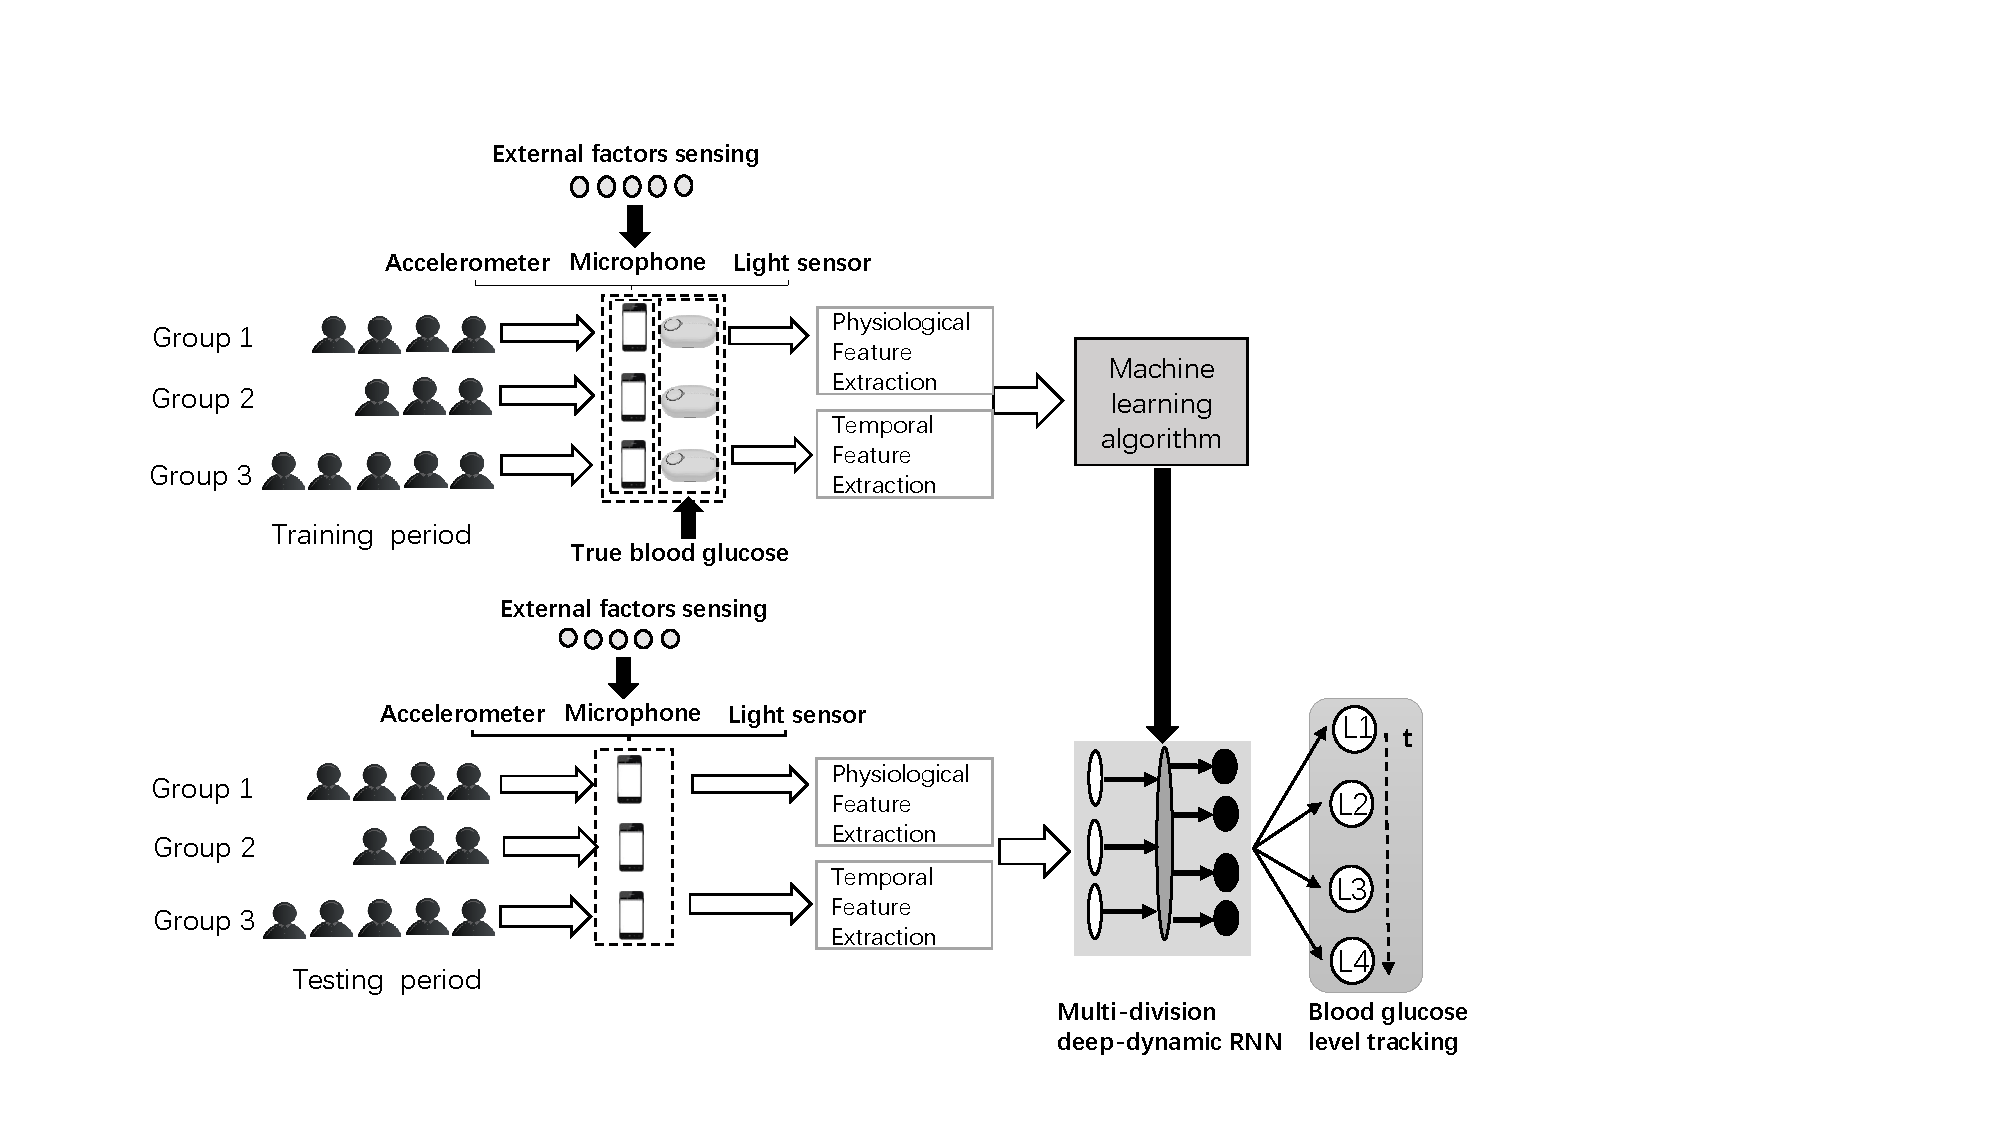
\includegraphics[width=0.85\columnwidth]{./img/System_Arch.pdf}
  \caption{Architecture of \sysname. \TODO{may need redraw}}
  \label{fig:architecture}
\end{figure}

\sysname is a smartphone-based blood glucose level tracking system that \emph{(i)} collects important external impacting factors, \emph{(ii)} efficiently trains a personalized blood glucose level model via a multi-task deep learning framework (\modelname), and \emph{(iii)} timely reminds users of abnormal blood glucose levels.
\figref{fig:architecture} shows the architecture of \sysname, which consists of three modules.

The \textbf{external factor collection} module records important factors that are important to infer blood glucose concentration and convenient to input via smartphones.
The only involvement required for users is the recording of their basic information (\eg health status, age, weight), record drug, insulin and food intake. As such, a user-friendly interface is designed to decompose the input process into multiple menu selections.
Meanwhile, \sysname will automatically measure the physical activities and sleep quality of the user via embedded sensors.
After collecting data from multiple users, the \textbf{multi-task deep learning} framework (\modelname) first learns feature representations from users in the same group (non-diabetic, type I and type II diabetic), and then adopts a deep RNN layer to learn a general blood glucose level model on the dataset of all users.
Finally it outputs a personalized blood glucose level model for each individual via a personality layer.
The \textbf{blood glucose level tracking} module takes measurements of the external factors as input, process the information with the trained personalized blood glucose level model, and finally outputs a specific blood glucose level at each time stamp.
In \sysname, we consider 4 blood glucose levels as in \tabref{tab:blood_glucose_levels}.

\begin{table}[h]
  \centering
  \caption{Normal and abnormal blood glucose levels~\cite{bib:BGWiKi}. The normal blood glucose concentration ranges from 4.4 mmol/L to 6.1 mmol/L. The blood glucose can grow to 7.8 mmol/L after eating. Blood glucose above 7.8 mmol/L for a prolonged period indicates the risk of diabetes mellitus. Blood glucose below 4.4 mmol/L is a sign of hypoglycemia.}
  \label{tab:blood_glucose_levels}
  \begin{tabular}{|c|c|c|}
  \hline
  \textbf{Blood Glucose Value (mmol/L)} & \textbf{Glocose Level} & \textbf{Explanation}                      \\ \hline
  (0, 4.4{]}                            & Level 1                & Low blood glucose (hypoglycemia)         \\ \hline
  (4.4, 6.1{]}                          & Level 2                & Normal level of fasting blood glucose      \\ \hline
  (6.1, 7.8{]}                          & Level 3                & Normal level of postprandial blood glucose \\ \hline
  (7.8, $+\infty$)                      & Level 4                & High blood glucose (hyperglycemia)          \\ \hline
  \end{tabular}
\end{table}


%The framework of \sysname is shown as \figref{fig:architecture}, consisting of four major components.
%The first one is the external factors collection.
%The users are required to enter their basic information into application, including of the age, the gender, the diabetes type and the year of diagnosis.

%After a user measures his/her blood glucose by a CGM, the records of the blood glucose along with the outer contextual factors occurred during the measurement are uploaded to an individual database automatically.
%Afterwards, a RNN model is trained based on the dataset to establish the relationships between the outer contextual factors and the corresponding blood glucose level.
%It then is fed into the user's smartphone.
%When the user does not wear the CGM, \sysname detects the outer contextual factors with embedded sensors in the smartphones, and infers the current blood glucose level based on the trained model.
%Once \sysname detects the abnormal points of blood glucose ( \ie in a \emph{high} or \emph{low} blood glucose level ), it reminds the user to measure the blood glucose by a clinical CGM for a further control.

%The extraction mechanisms of outer contextual factors are detailed as follows.
%
%\emph{Physical activity}:
%\sysname leverages the accelerometer to detect the user's activities by the approaches in \cite{bayat2014study}, as well as the corresponding time costs.
%\sysname then measures the calorie of user's physical consumption.
%
%\emph{Food intake}:
%\sysname measures the food's effect on a person's blood glucose level based on the glycemic index.
%
%\emph{Clinical drug intake}:
%\sysname records the name and amount of the drug that user eat.
%
%\emph{Time}:
%\sysname invokes the timer embedded in the smartphone to record the time.
%
%\emph{Sleep quality}:
%\sysname measures the user's sleep by the approach in \cite{gu2014intelligent}.


\section{Design}
\label{sec:design}

\subsection{External factor collection}
\label{subsec:external}
Sensing module is mainly designed for collected the external factors of users.

\paragraph{Food intake}
As the food intake is a main source of carbohydrate, \sysname provides the food menu for users to record their daily intakes based on the carbohydrate food list \cite{bib:carblist}.
Five common food categories have been provided by \sysname, including grains ,vegetables, mike and egg,fruits and meats. The users are asked to enter their food items and the corresponding amounts. \sysname calculate the carbohydrate of a meal and measure its impact on blood glucose level.

\paragraph{Drug intake}
The oral diabetes medications enhance secretion of insulin into the blood by the pancreas or decrease amount of glucose released from liver, keeping the blood glucose in a low level for type II diabetes.
In \sysname, a drug menu of 11 oral diabetes is report for users to input their drug intake. After eating the diabetes drugs, users select their pills name and report the drug dosage. The drug list is provided based on \cite{bib:druglist}.
\sysname transfers the drug dose as the blood glucose efforts according to their work functions \cite{bib:druglist, bib:bolen2007systematic, bib:bennett2011oral}  by physiological model.

\paragraph{Insulin injection}
Insulin injection is to control blood glucose concentration of those who have type I diabetes, and the patients of type II, whose blood sugar is too high for their bodies to control. \sysname provides a insulin type list based on \cite{bib:insulinlist} for user with diabetes to enter their usage and insulin dosage, and then transfer it into physiological model to compute the blood glucose level.

\paragraph{Activity factors}
Since the carbohydrate in the body can be consumed by daily exercise, resulting to varying the blood glucose level, \sysname adopts an effective and power efficient approach \cite{bib:kwapisz2011activity} to automatically recognize six common user's daily activities (i.e., walking, running, upstairs, downstairs, sitting and standing), and record the corresponding durations. The caloric expenditure can be easily consumed by the calorie burn calculator formulas as Equation ~\ref{calorie_burn}.
\begin{equation}\label{calorie_burn}
  Calorie Burn = (BMR/24)*MET*T,
\end{equation}
where BMR (Basal Methobolic Rate) is the amount of energy required to simply sit or lie quietly \cite{bib:mcnab1997utility}, and MET (Metabolic Equivalent) is the ratio of the work metabolic rate to the resting metabolic rate\cite{bib:ainsworth2000compendium}. The calculator formula has been widely used by multiple sport applications \cite{bib:shapesense, bib:HealthStatus, bib:CalorieCounter}.
\sysname finally leverages the calories to measure the effects of exercise on the blood glucose.

\paragraph{Sleep quality}
Sleep quality has a long influence on blood glucose level. To measure the sleep quality of users, \sysname applies an effective method in \cite{bib:gu2014intelligent} to measure the sleep quality, and leverages the sleep quality score as an index to evaluate the sleeping impact on blood glucose level.

\subsection{Feature Engineering of Physiological-Temporal Views }
\subsubsection{Physiological View}
The feature engineering of physiological view is used to describe the variance of inner body physiological factors. The principal physiological impact factors are composed of carbohydrate

\subsection{Blood glucose level prediction}

% !TEX root = paper.tex

\subsection{Intuition}
Given the features extracted from the physiological process, it seems plausible to perform any classification algorithm for blood glucose level prediction. Nonetheless, this plug-and-play approach will neglect important information from (1) dynamics of the process, and (2) inter-user similarity among same group of participants. Traditionally, various sequential classification methods[], e.g., hidden Markov model (HMM), recurrent neural networks (RNN), and dynamic conditional random fields (CRF), are used to capture the temporal correlation of the input feature. The inter process correlations are often times incorporated with the so-called multi-task learning approaches[], which learns processes (or tasks) in parallel to improve classification or to reduce the data sample requirement. 

In this paper, a novel machine learning paradigm, namely Multi-division deep-dynamic RNN (Md$^3$RNN), is proposed. To include the the aforementioned information sources in an unified framework, we develop two key ideas that extend the classical RNN. Firstly, the single hidden layer in RNN is replaced with several deep stacked layers. The deep structure in the new model is able to describe complex, mutli-scale system dynamics that would otherwise be ignored (or averaged out) by prior ``shallow'' models such as HMM, RNN, and CRF. Secondly, the correlations among users, being quite significant within user groups (divisions), are encoded by group-shared input layer and common hidden layers, whereas the distinct characteristics of individual users are modeled with  different output layers for personalized prediction. Within a larger scope of machine learning, the proposed Md$^3$RNN aims to leverage recent advancement of deep learning and multi-task learning, to model group-interacted time series data having complex temporal dynamics. It can be viewed as both a deep extension of RNN, and an intermediate between single-task learning and multi-task learning, hence the name Md$^3$RNN.

The overall configuration of the proposed model is summarized in Fig.\ref{fig:rnn}. Detailed construction of each component is given in the sequel.     

\begin{figure}[!t]
  \centering
  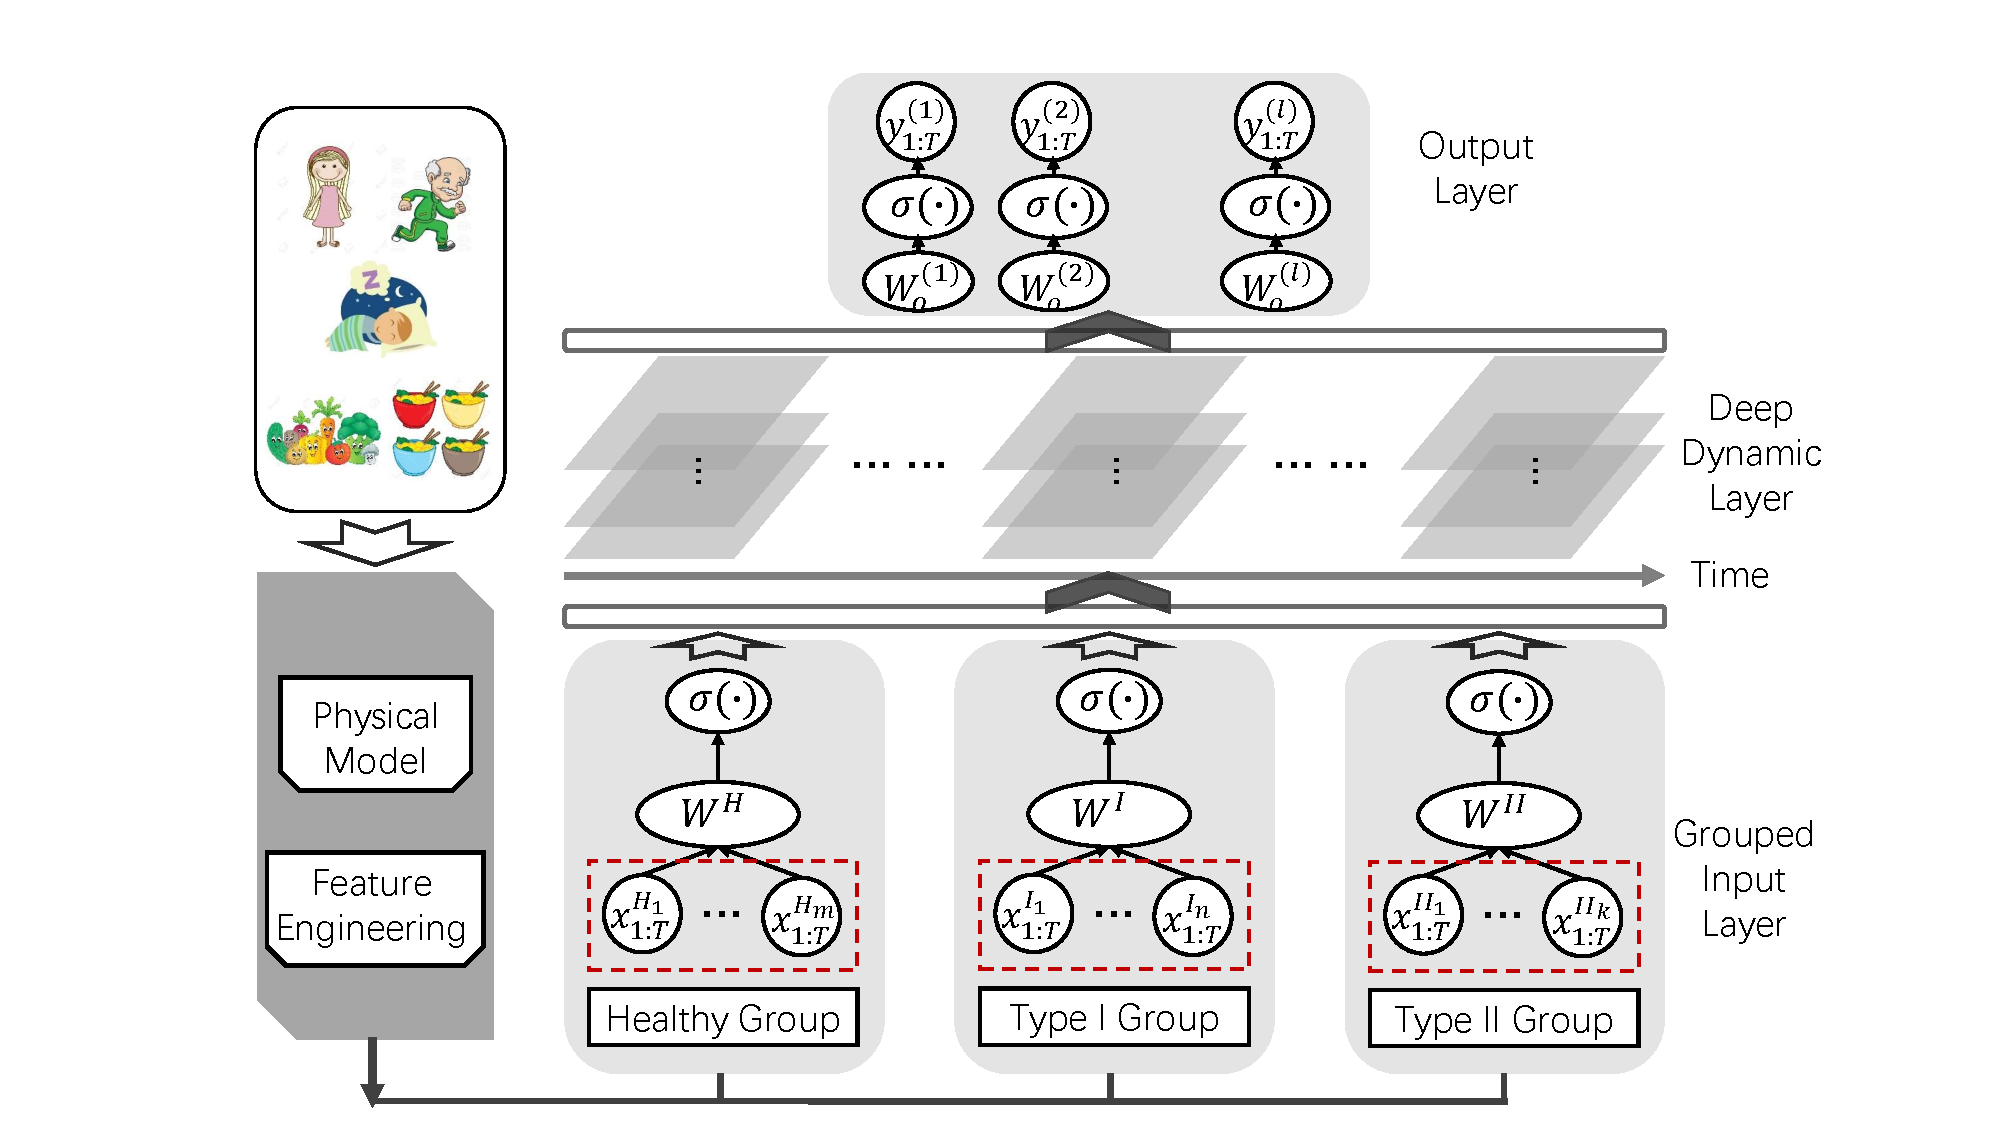
\includegraphics[width=0.9\columnwidth]{./img/pics_RNN.pdf}
  \caption{The Md$^3$RNN structure}
  \label{fig:rnn}
\end{figure}

\subsection{Model construction by layers}
The input of the Md$^3$RNN are the features extracted from the physiological model. The labeled data sequences for user number $j$ at time $t$ are denoted by $(x_i^{j},y_i^{j})$. We also adopt an index set convention, that $(x_A^{B},y_A^B)$ represents the data set $\left\{(x_i^{j},y_i^{j}) | i \in A, j\in B\right\}$ given index sets $A$ and $B$.
\subsubsection{Grouped Input Layer}
In the context of blood glucose prediction, available inputs are naturally divided into three groups according to the health condition of the participant from whom the data was generated. Notation-wise, we utilize $H$, $I$ and $II$ to indicate the the group of healthy user, user with type I diabetes and those having type II diabetes, respectively. Since the extracted features are essentially physiological indexes of an ``average'' person, they must go though different transformations to represent useful information of three distinct groups. This consideration motivate the design of the input layer (bottom of Fig.\ref{fig:rnn}) - it is divided into three units that performs different linear and non-linear transformation according to user groups. For instant, a data sample $x_t^{I_j}$, generated at time $t$ from the $j^{th}$ user of type I, undergoes the following processing:
\begin{align}
\tilde{x}_t^{I_j} = \sigma \left( W^Ix_t^{I_j} \right)
\end{align}     
where $W^I$ is the coefficients of the affine transformation \footnote{We assume that the interception is included in $W$. This can be done by simply adding a feature of all $1$s.}, $\sigma$ is some activation function, and $\tilde{x}_t^{I_j}$ is the output of the input layer for that data sample. Similar operations are conducted for data samples from group $H$ and $II$, but with different transformation coefficients. Intuitively, the shared transformation within groups would improve the learning of parameters (vs. single task learning), as information from all data in a homogeneous group is used. Also, the transformation can be stacked into several (say $P$) layers, for better information representation.   

\subsubsection{Deep Dynamic Layer}
A common hidden layer is designated to capture the dynamics of the blood glucose evolution process. The underlying assumption is that, the biological and chemical reactions governing blood glucose variation are similar for all people, despite of grouped behaviors in the representation of physiological indexes (input layer), or individual characteristics in exhibited glucose level. This assumption could be justified by a series of medical research[][]. Moreover, since all users share the same hidden layer, all collected data samples are eventually helping the estimation of its parameters. The availability of rich information for the hidden layer makes the learning of a deep structure possible. In Md$^3$RNN, a number of Long Short Term Memory (LSTM) networks are stacked together (middle of Fig.\ref{fig:rnn}), to increase the overall model flexibility. In particular, it has been justified in both theory and practice that stacked LSTMs are able to capture dynamics occurring at different time scales, which in the current application would enable the modeling of both slow and rapid biological/chemical reactions. Although a wide variety of LSTM configuration exist in literature, in this work we adopt the one recently proposed by [], which combines the forget/input gate and merges cell/hidden state for simplicity and better generalization performance. Mathematically, given the output from the grouped input layer, the deep dynamic layer performs
\begin{equation}
\begin{aligned}
&z^d_t = \sigma\left( W^d_z [h_{t-1}^d,h_t^{d-1}] \right) \\
&r^d_t = \sigma\left( W^d_r [h_{t-1}^d,h_t^{d-1}] \right) \\
&\tilde{h}_t^d = tanh\left( W^d_h [r_t^d*h_{t-1}^d,h_t^{d-1}] \right) \\
&h^d_t = (1-z_t^d)*h_{t-1}^d + z_t^d*\tilde{h}_t^d
\end{aligned}
\end{equation}
for hidden layer numbered $d = 1,2,\cdots,D$. At the first dynamic layer with $d=1$, the input $h_t^{d-1}$ is set to be the output from the grouped input layer, and the output of the last dynamic layer, $h^D_t$, will be used as the input of the last component of Md$^3$RNN. 

\subsubsection{Personalized Output Layer}
Finally, each user is assigned a personalized output layer, parameterized by $W_o^j, j=1,\cdots,l$, which performs a single linear and softmax transformation on the results of the deep dynamic layer. The particular configuration of the output layer compensates for the individual characteristics in the exhibited blood glucose (i.e., measured blood glucose level). Because only data generated by a specific participant $j$ will have an effect on the its parameters $W_o^j$, the personalized output layer is set to have a ``shallow structure'', i.e., it only performs the transformation once. More specifically, given $h^D_t$ from user $j$, it computes
\begin{equation}
\hat{y}_t^j = \text{softmax} \left( W_o^j h^D_t \right)
\end{equation}

\subsection{Cost Sensitive Learning and Hyperparamter (Model) Selection}

Similar to other deep neural network learning, Md$^3$RNN is trained by minimizing the sum of losses over all the time steps. The definition of the loss function has much bearing on the generalization performance of the method. In particular for the current application, simply minimizing a general error rate seems inappropriate, because the costs of different types of misclassifiction errors are not the same. For example, missing the detection of high blood glucose (type I or II) is more costly than misclassifying normal condition to an alarm for high glucose. Moreover, in the collected data set from real people, the training data is inherently imbalanced - the available samples labeled Level 1 and Level 4 are much fewer (only 7\%) compared to samples in the other categories (Level 2 and Level 3). 

The above concerns motivate the cost sensitive learning of Md$^3$RNN. Instead of directly minimizing a surrogate of error rate, we propose to optimize over a weighted version of classification losses[]. More specifically, the following total loss function is considered:
\begin{equation}
L = \sum_{t} \sum_{y_t \in \mathcal{Y}} l(y_t,\hat{y}_t)C_{y_t}
\end{equation} 
where $\mathcal{Y}$ is the label set, and $\hat{y}_t$s are prediction output from Md$^3$RNN. Our implementation uses cross entropy for $l(y_t,\hat{y}_t)$, but generally the ``base'' lost function $l(y_t,\hat{y}_t)$ can be any surrogate of the error function. The additional coefficient $C_{y_t}$ weights the misclassification error for category $y_t$. In the current application, $\mathcal{Y} = \{1,2,3,4\}$, associated with four coefficients $C_1$ to $C_4$. Those cost weighting coefficients are treated as hyperparameters of the proposed model, but in other applications of Md$^3$RNN, they can also be determined with prior knowledge about the misclassification cost and the class imbalance. 

With the technique of back-propagating, computing the gradient of Md$^3$RNN is not so different from gradient calculation of classical RNN. In this work, we accomplish those computation using Tensorflow[], and proceed to learn Md$^3$RNN model by stochastic gradient descent for overall loss minimization.

Last but not least, the construction of the Md$^3$RNN model involves choosing 15 hyperparameters, e.g., cost coefficients $C_{y}$, depth $D$ of the stacked dynamic layer, learning rate, number of hidden unit in the input layer, etc. Direct application of cross validation (CV) for hyperparameter tuning, even with the help of parallel computing, seems endless as the number of required CVs scales exponentially to the number of hyperparameters. In this regards, we adopt Bayesian optimization (BO), a recent tool developed for blackbox function optimization with limited evaluations. The decision variables of BO are those hyperparameters, and the objective is the F-score of the precision and recall on some testing data set. Note that BO has been used recently for the hyperparameter (model) selection of many deep learning paradigms [][].            





\section{Evaluation}
\label{sec:eval}
\subsection{Experimental Settings}
\subsubsection{Datasets}
We built our blood glucose dataset from July 2016 to January 2017. A total of 112 users joined in our experiments. Table~\ref{dataset} illustrates the details of the dataset.
\begin{itemize}
  \item Blood Glucose Data: During the experiments, each user wears a CGM device to collect the blood glucose sample every 3 minutes. \sysname divides the blood glucose value into four levels by preset thresholds. The numbers of blood glucose samples in each level are shown in Table~\ref{dataset}. In our experiments, all the users are promise to wear CGM for at least 5 days. The distribution of experimental durations are listed in Table~\ref{dataset}.
  \item External Factors Data: In the duration of wearing the CGM, each user installs \sysname on smartphone to sense the daily activities and sleep quality automatically. Meanwhile, users also leverage \sysname to record their daily meals, drug and insulin input. \sysname transfers the external factors as variables of physiological model at corresponding time.
  \item User Basic Information Data: The users are required to record the basic personal data relevant to blood glucose (e.g., age, weight, gender and health status) into \sysname, which are listed in Table~\ref{dataset}. \sysname classifies the users into three groups based on their health status.

\end{itemize}





\begin{table}[]
\centering
\caption{The Details of Dataset}
\label{dataset}
\begin{tabular}{clccclcccccl}
\hline\hline
\multicolumn{12}{c}{\textbf{Blood Glucose}}                                                                                                                                                                                               \\ \hline
\multicolumn{2}{l}{\textbf{\cellcolor[gray]{0.8}Blood Level}} & \multicolumn{2}{r}{\textbf{\cellcolor[gray]{0.8}Level 1}} & \multicolumn{2}{c}{\textbf{\cellcolor[gray]{0.8}Level 2}} & \multicolumn{2}{c}{\textbf{\cellcolor[gray]{0.8}Level 3}} & \multicolumn{2}{c}{\textbf{\cellcolor[gray]{0.8}Level 4}} & \multicolumn{2}{c}{\textbf{\cellcolor[gray]{0.8}Total}} \\
\multicolumn{2}{l}{Number of Sample}     & \multicolumn{2}{c}{75369}            & \multicolumn{2}{c}{293530}           & \multicolumn{2}{c}{235686}           & \multicolumn{2}{c}{158054}           & \multicolumn{2}{c}{762639}         \\ \hline\hline
\multicolumn{12}{c}{\textbf{Experimental Duration}}                                                                                                                                                                                          \\ \hline
\multicolumn{2}{l}{\textbf{\cellcolor[gray]{0.8}Days}}        & \multicolumn{2}{c}{\textbf{\cellcolor[gray]{0.8}6-10}}    & \multicolumn{2}{c}{\textbf{\cellcolor[gray]{0.8}11-15}}   & \multicolumn{2}{c}{\textbf{\cellcolor[gray]{0.8}16-20}}   & \multicolumn{2}{c}{\textbf{\cellcolor[gray]{0.8}21-25}}   & \multicolumn{2}{c}{\textbf{\cellcolor[gray]{0.8}26-30}} \\
\multicolumn{2}{l}{Number of Users}      & \multicolumn{2}{c}{48}               & \multicolumn{2}{c}{24}               & \multicolumn{2}{c}{20}               & \multicolumn{2}{c}{13}               & \multicolumn{2}{c}{7}              \\ \hline\hline
\multicolumn{12}{c}{\textbf{User Basic Information}}                                                                                                                                                                                      \\ \hline
\multicolumn{2}{l}{\textbf{\cellcolor[gray]{0.8}Age}}         & \multicolumn{2}{c}{\textbf{\cellcolor[gray]{0.8}15-24}}   & \multicolumn{2}{c}{\textbf{\cellcolor[gray]{0.8}25-34}}   & \multicolumn{2}{c}{\textbf{\cellcolor[gray]{0.8}35-44}}   & \multicolumn{2}{c}{\textbf{\cellcolor[gray]{0.8}45-54}}   & \multicolumn{2}{c}{\textbf{\cellcolor[gray]{0.8}55-70}} \\
\multicolumn{2}{l}{Number of Users}      & \multicolumn{2}{c}{8}                & \multicolumn{2}{c}{17}               & \multicolumn{2}{c}{24}               & \multicolumn{2}{c}{29}               & \multicolumn{2}{c}{34}             \\
\multicolumn{2}{l}{\textbf{\cellcolor[gray]{0.8}Weight}}      & \multicolumn{2}{c}{\textbf{\cellcolor[gray]{0.8}30-44}}   & \multicolumn{2}{c}{\textbf{\cellcolor[gray]{0.8}45-54}}   & \multicolumn{2}{c}{\textbf{\cellcolor[gray]{0.8}55-64}}   & \multicolumn{2}{c}{\textbf{\cellcolor[gray]{0.8}65-74}}   & \multicolumn{2}{c}{\textbf{\cellcolor[gray]{0.8}75-90}} \\
\multicolumn{2}{l}{Number of Users}      & \multicolumn{2}{c}{18}               & \multicolumn{2}{c}{21}               & \multicolumn{2}{c}{32}               & \multicolumn{2}{c}{22}               & \multicolumn{2}{c}{19}             \\
\multicolumn{4}{l}{\textbf{\cellcolor[gray]{0.8}Gender}}      & \multicolumn{3}{c}{\textbf{\cellcolor[gray]{0.8}Male}}                                                               & \multicolumn{5}{c}{\textbf{\cellcolor[gray]{0.8}Female}}                                                          \\
\multicolumn{4}{l}{Number of Users}      & \multicolumn{3}{c}{57}                                                                          & \multicolumn{5}{c}{55}                                                                       \\ \hline\hline
\multicolumn{12}{c}{\textbf{User Health Status}}                                                                                                                                                                                          \\ \hline
\multicolumn{3}{l}{\textbf{\cellcolor[gray]{0.8}Health Status}}                   & \multicolumn{3}{c}{\textbf{\cellcolor[gray]{0.8}Health}}                     & \multicolumn{3}{c}{\textbf{\cellcolor[gray]{0.8}Type I}}                      & \multicolumn{3}{c}{\textbf{\cellcolor[gray]{0.8}Type II}}                  \\
\multicolumn{3}{l}{Number of Users}                          & \multicolumn{3}{c}{35}                                  & \multicolumn{3}{c}{38}                                   & \multicolumn{3}{c}{39}                                \\ \hline
\end{tabular}
\end{table}



\subsubsection{Ground Truth and Metrics}

The blood glucose samples collected by the CGM are regarded as groundtruth. We compare the prediction results of \sysname with the groundtruth, and the performance is measured in terms of the precision \cite{}, recall\cite{} and accuracy\cite{}.






%
%
%\begin{table}[]
%\centering
%\caption{The details of dataset}
%\label{The details of dataset}
%\begin{tabular}{|l|c|c|c|c|l|}
%\hline
%\textbf{Blood Level}                  & \textbf{Level 1} & \textbf{Level 2} & \textbf{level 3} & \textbf{Level 4} & \textbf{Total}         \\ \hline
%\multicolumn{1}{|c|}{\textbf{Number}} & 75369            & 293530           & 235686           & 158054           & \multicolumn{1}{c|}{762639} \\ \hline
%\end{tabular}
%\end{table}















\begin{table}[]
\centering
\caption{Confusion matrix of \sysname performance}
\label{tab:confusion_matrix}
\begin{tabular}{|c|c|c|c|c|l|l|}
\hline
\multirow{2}{*}{\textbf{\begin{tabular}[c]{@{}c@{}}Ground\\ Truth\end{tabular}}} & \multicolumn{4}{c|}{\textbf{Predictions}}                                                                                 & \multicolumn{2}{l|}{\multirow{2}{*}{}}                                                            \\ \cline{2-5}
                                                                                 & Level 1                      & Level 2                      & Level 3                      & Level 4                      & \multicolumn{2}{l|}{}                                                                             \\ \hline
Level 1                                                                          & \cellcolor[gray]{0.8}62657                        & 5521                         & 3672                         & 3519                         & 83.13\%                             & \multirow{4}{*}{\rotatebox{90}{\textbf{Recall}} }                           \\ \cline{1-6}
Level 2                                                                          & 16346                        &  \cellcolor[gray]{0.8}240584                       & 27563                        & 9037                         & 81.96\%                             &                                                             \\ \cline{1-6}
Level 3                                                                          & 2660                         & 30905                        & \cellcolor[gray]{0.8}188472                       & 13649                        & 79.97\%                             &                                                             \\ \cline{1-6}
Level 4                                                                          & 3443                         & 5620                         & 14278                        & \cellcolor[gray]{0.8}134713                       & 85.23\%                             &                                                             \\ \hline
\multicolumn{1}{|l|}{\multirow{2}{*}{}}                                          & \multicolumn{1}{l|}{73.62\%} & \multicolumn{1}{l|}{85.12\%} & \multicolumn{1}{l|}{80.55\%} & \multicolumn{1}{l|}{83.72\%} & \multicolumn{2}{l|}{\multirow{2}{*}{\begin{tabular}[c]{@{}l@{}}Accuracy:\\ 82.14\%\end{tabular}}} \\ \cline{2-5}
\multicolumn{1}{|l|}{}                                                           & \multicolumn{4}{c|}{\textbf{Precision}}                                                                                 & \multicolumn{2}{l|}{}                                                                             \\ \hline
\end{tabular}
\end{table}



\subsubsection{System Evaluation}

To evaluate the \sysname performance, we provide CGM for each new user for one time usage, supporting more than 5 days. We take the former 4 days as the training data, and left days as the testing data. If the left days of one users are longer than 2 days, we calculate the user's average performance. Table~\ref{tab:confusion_matrix} shows the results of testing dataset. As we can see,  the recalls of four blood glucose levels are above 79\%, and all the precisions of four blood glucose levels keep above 73\%. In particular, the recalls of level 1 and level 3 are 83.13\% and 85.23\%, demonstrating the high sensitivity of \sysname towards these two levels. The 82.14\% accuracy states the outstanding prediction performance of \sysname.


\subsubsection{Evaluation on Multi-task Model structure}
To demonstrate the effectiveness of \modelname structure, we compared our model over the following combinations.

\begin{itemize}

  \item \emph{General Learning}:
  All the users shared a same information representation, dynamic and personality layers, which assumes the blood glucose trends of all users can be tracked by a same model.


  \item \emph{Single Learning }:
  Each user is trained for a specific model.

  Fig.~\ref{fig:cmp_model} shows the results.
\end{itemize}


\begin{figure}[!t]
\centering
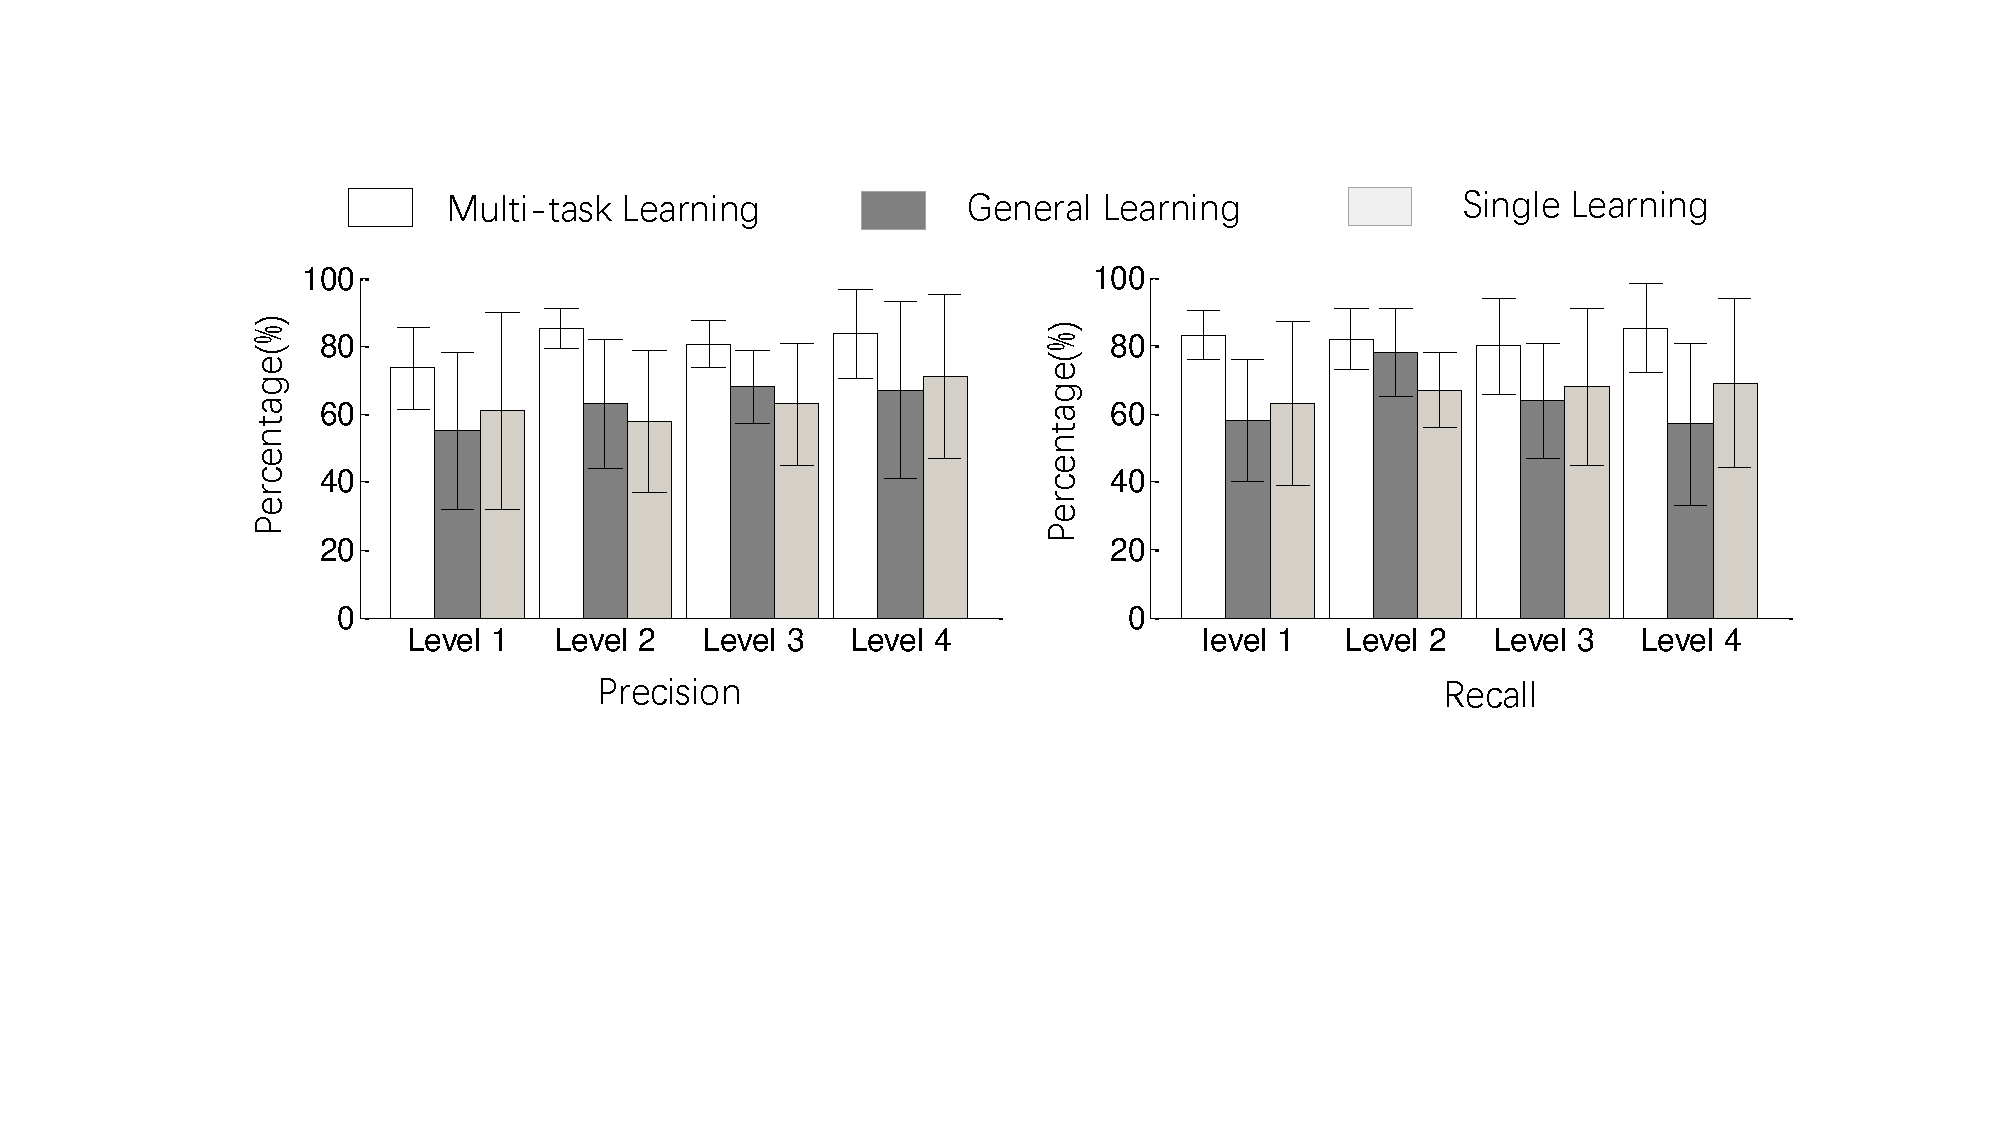
\includegraphics[width=0.9\columnwidth]{./img/CMP_Models.pdf}
\caption{The model comparison}
\label{fig:cmp_model}
\end{figure}


\subsubsection{Multi-task Model and General Model Comparison in Group}
We also apply general learning approach on the users in same group, and compare the prediction performance of \modelname. Fig.~\ref{fig:cmp_groups}
shows the results. As is shown, \modelname outperforms the general learning methods in each group, especially the performance of level 1 and level 4. It mainly results by two reasons. On the one hand, the limitation of blood glucose data in each group weakens the capability of temporal dynamic characteristics. On the other hand, the imbalanced distribution of blood glucose data of one group also low the performance down. For example, much more data of level 4 and much less data of level 1 in group 3 (type II diabetes) low down the recall of level 1 and the precision of level 4. It is even hard to be solved by the cost sensitive approach.


\begin{figure}[!t]
\centering
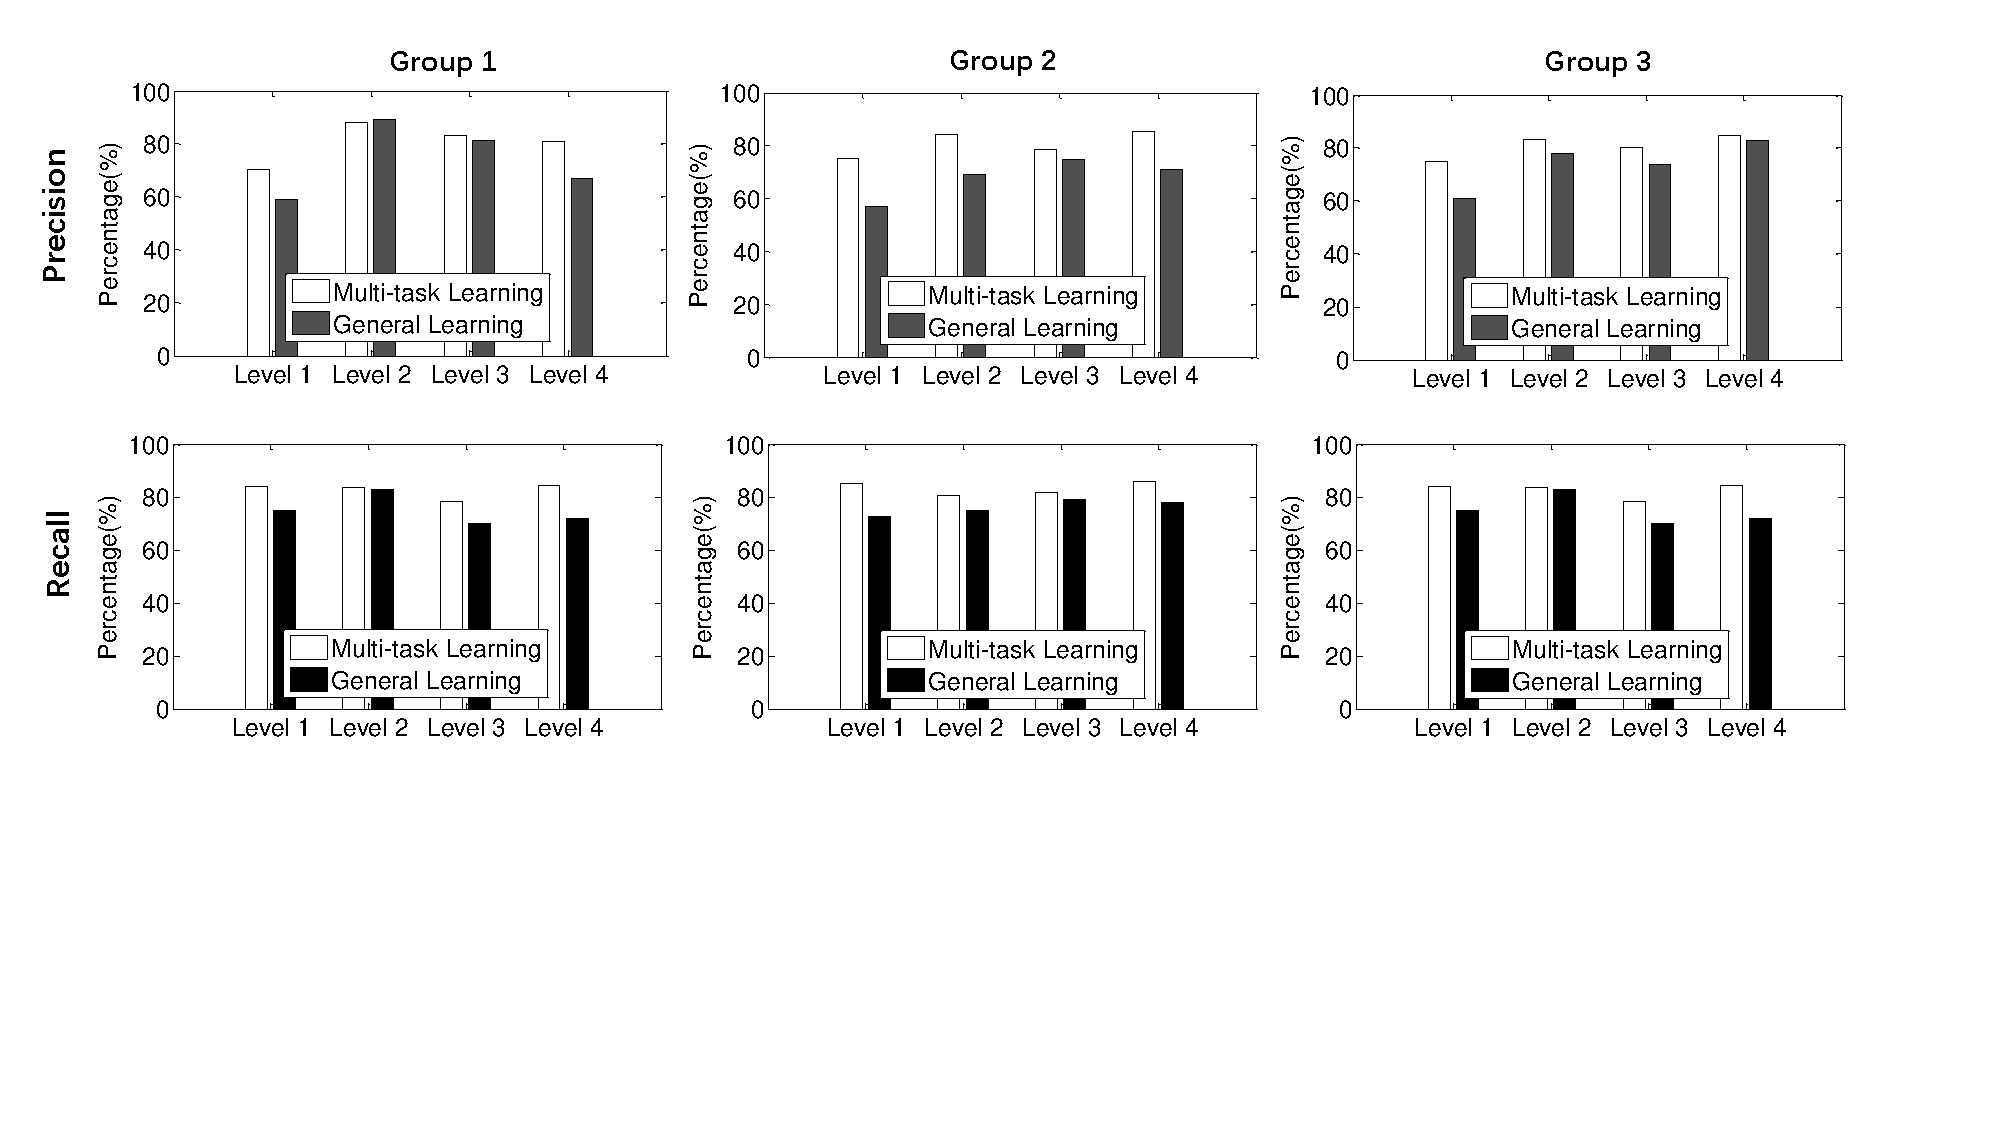
\includegraphics[width=0.9\columnwidth]{./img/group_multi_task.pdf}
\caption{The comparison of multi-task learning and group general learning.}
\label{fig:cmp_groups}
\end{figure}


\subsubsection{Evaluation with various training data}

Since the users may wear CGM continuously, we evaluate the performance of \sysname with increasement of training dataset by five days. Under each system evaluation, we trained all the data of the users with before the testing date, and measured the system by calculating the average performance of those who have longer testing days.

Fig.~\ref{fig:per_under_train_days} illustrates the results. We can see the system performance grow up with the increasement of training dataset, demonstrating the performance of \sysname will grow up with more training data.


\begin{figure}[!t]
\centering
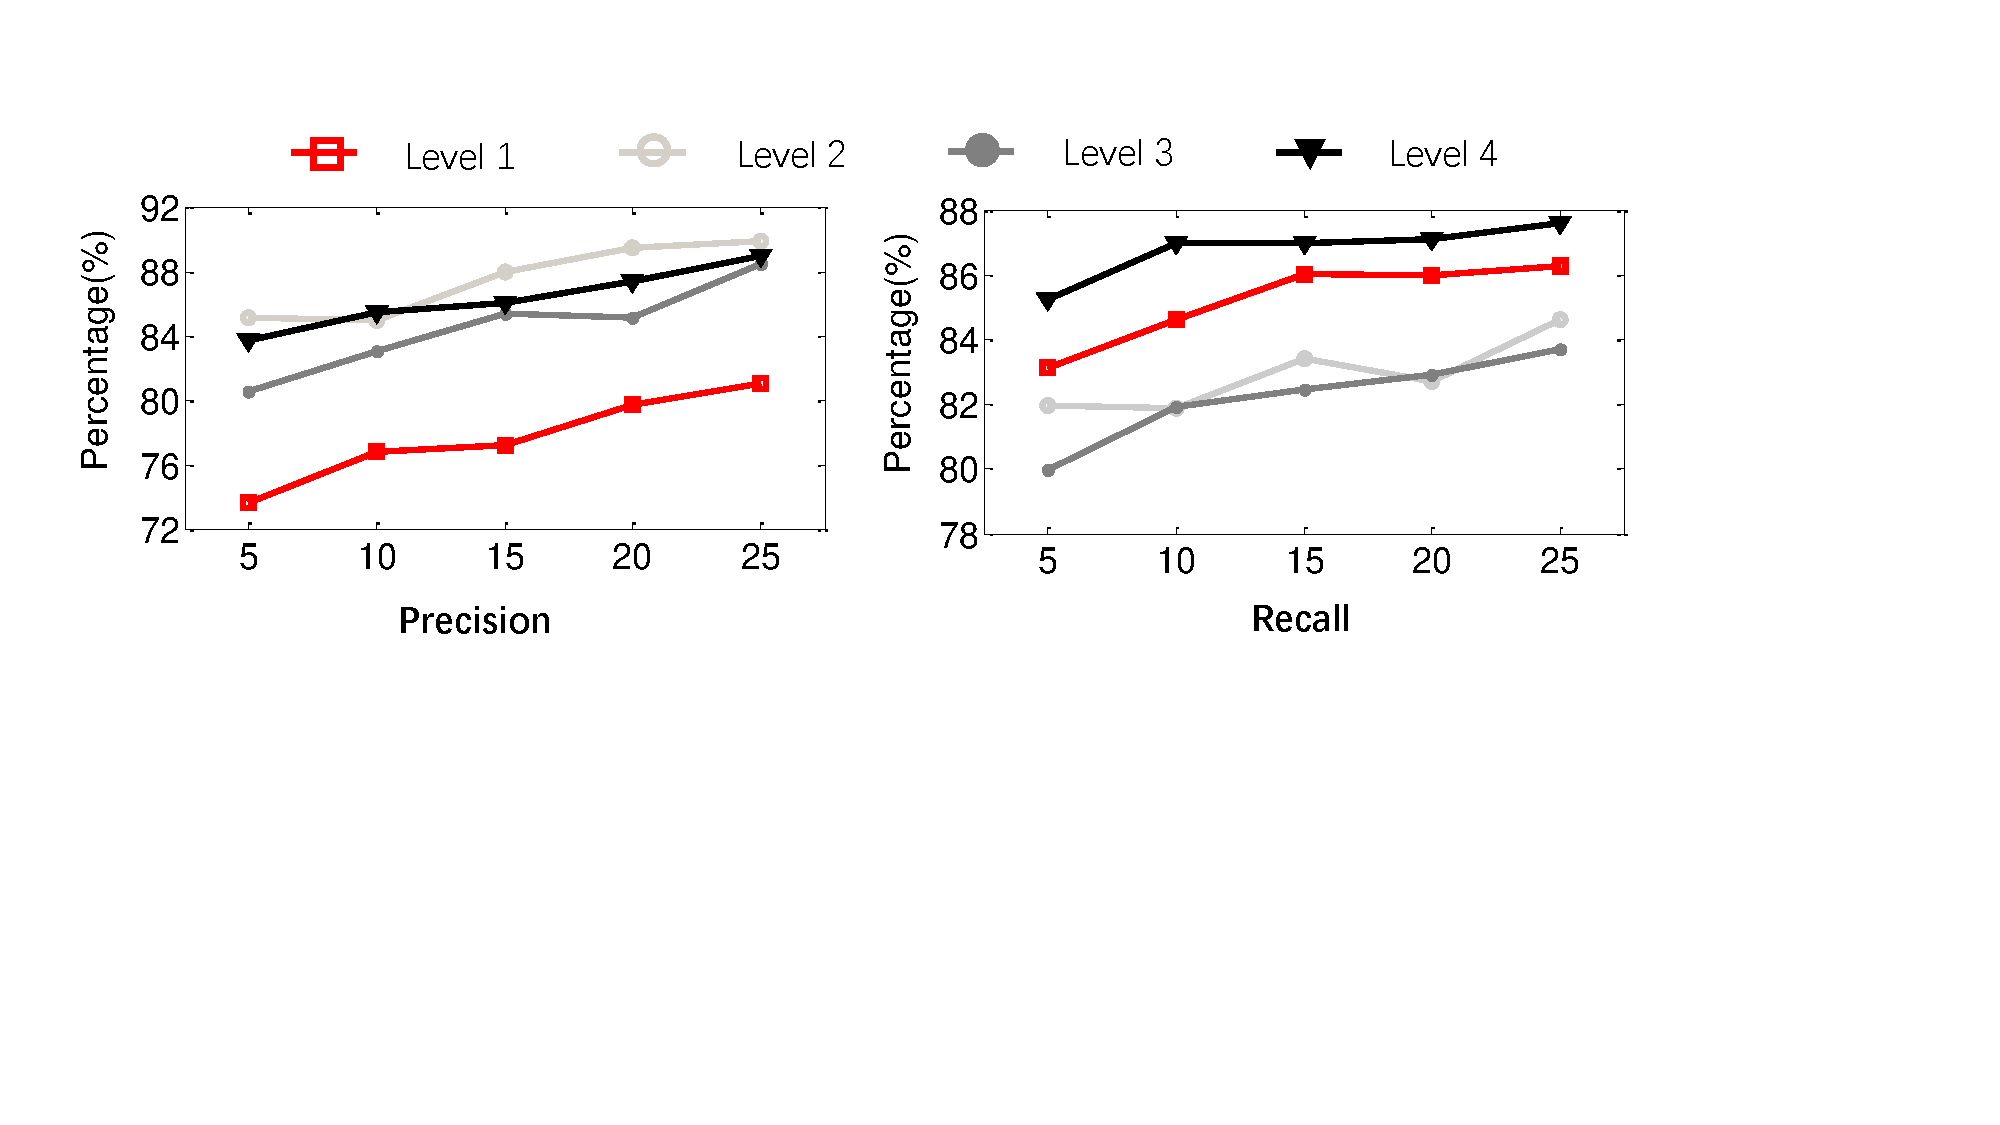
\includegraphics[width=0.9\columnwidth]{./img/performance_under_days.pdf}
\caption{System performance under different training date}
\label{fig:per_under_train_days}
\end{figure}



\paragraph{Evaluation with various prediction duration}

Considering the uncertainties of blood glucose increase while the time passing by, we detail the system performance by differentiating the prediction durations in  Fig.~\ref{fig:per_under_various_pred_days}.
As expected, the system performance shows a decrease trend while the prediction duration leave longer away. It is possible due to the internal relevant factors of blood glucose changed with the time passing by. However, the system performance still can maintain an acceptable level for 30-days prediction.



\begin{figure}[!t]
\centering
\includegraphics[width=0.9\columnwidth]{./img/Performance under prediction
longer.pdf}
\caption{System performance under different prediction duration}
\label{fig:per_under_various_pred_days}
\end{figure}



\subsubsection{Evaluation on Features}

We show the effectiveness of four-dimensional feature in Table ~\ref{Feature_Evaluation}. Clearly, the tracking performance of \sysname improve a lot by adding one feature set into the model.



\begin{table}[]
\small
\centering
\caption{Feature Evaluation}
\label{Feature_Evaluation}
\begin{tabular}{|c|c|c|c|c|c|c|c|c|}
\hline
                                   & \multicolumn{2}{c|}{\textbf{Level 1}}                     & \multicolumn{2}{c|}{\textbf{Level 2}} & \multicolumn{2}{c|}{\textbf{Level 3}}                     & \multicolumn{2}{c|}{\textbf{Level 4}}                     \\ \hline
\textbf{Features}                  & \textbf{Precision} & \multicolumn{1}{l|}{\textbf{Recall}} & \textbf{Precision}  & \textbf{Recall} & \textbf{Precision} & \multicolumn{1}{l|}{\textbf{Recall}} & \textbf{Precision} & \multicolumn{1}{l|}{\textbf{Recall}} \\ \hline
$F_{p}$                            & 43.37$\%$               & 32.82$\%$                                 & 46.03$\%$                & 39.10$\%$            & 51.79$\%$               & 48.95$\%$                                 & 56.30$\%$               & 43.49$\%$                                 \\ \hline
$F_{p}$+$F_{t1}$                   & 51.97$\%$               & 58.11$\%$                                 & 60.42$\%$                & 58.90$\%$            & 63.35$\%$               & 53.59$\%$                                 & 69.82$\%$               & 55.16$\%$                                 \\ \hline
$F_{p}$+$F_{t1}$+$F_{t2}$          & 64.60$\%$               & 73.08$\%$                                 & 69.87$\%$                & 61.23$\%$            & 74.33$\%$               & 67.81$\%$                                 & 76.64$\%$               & 72.32$\%$                                 \\ \hline
$F_{p}$+$F_{t1}$+$F_{t2}$+$F_{t3}$ & 73.62$\%$   & 83.13$\%$                                 & 83.13$\%$               & 83.13$\%$            & 80.55$\%$   & 79.97$\%$
& 83.72$\%$               & 85.23$\%$                                  \\ \hline
\end{tabular}
\end{table}


\subsubsection{Blood glucose level predictions}

Fig.~\ref{fig:pre_gt} compares the predictive results of \sysname and true blood glucose level of a user over one day.






\begin{figure}[!t]
\centering
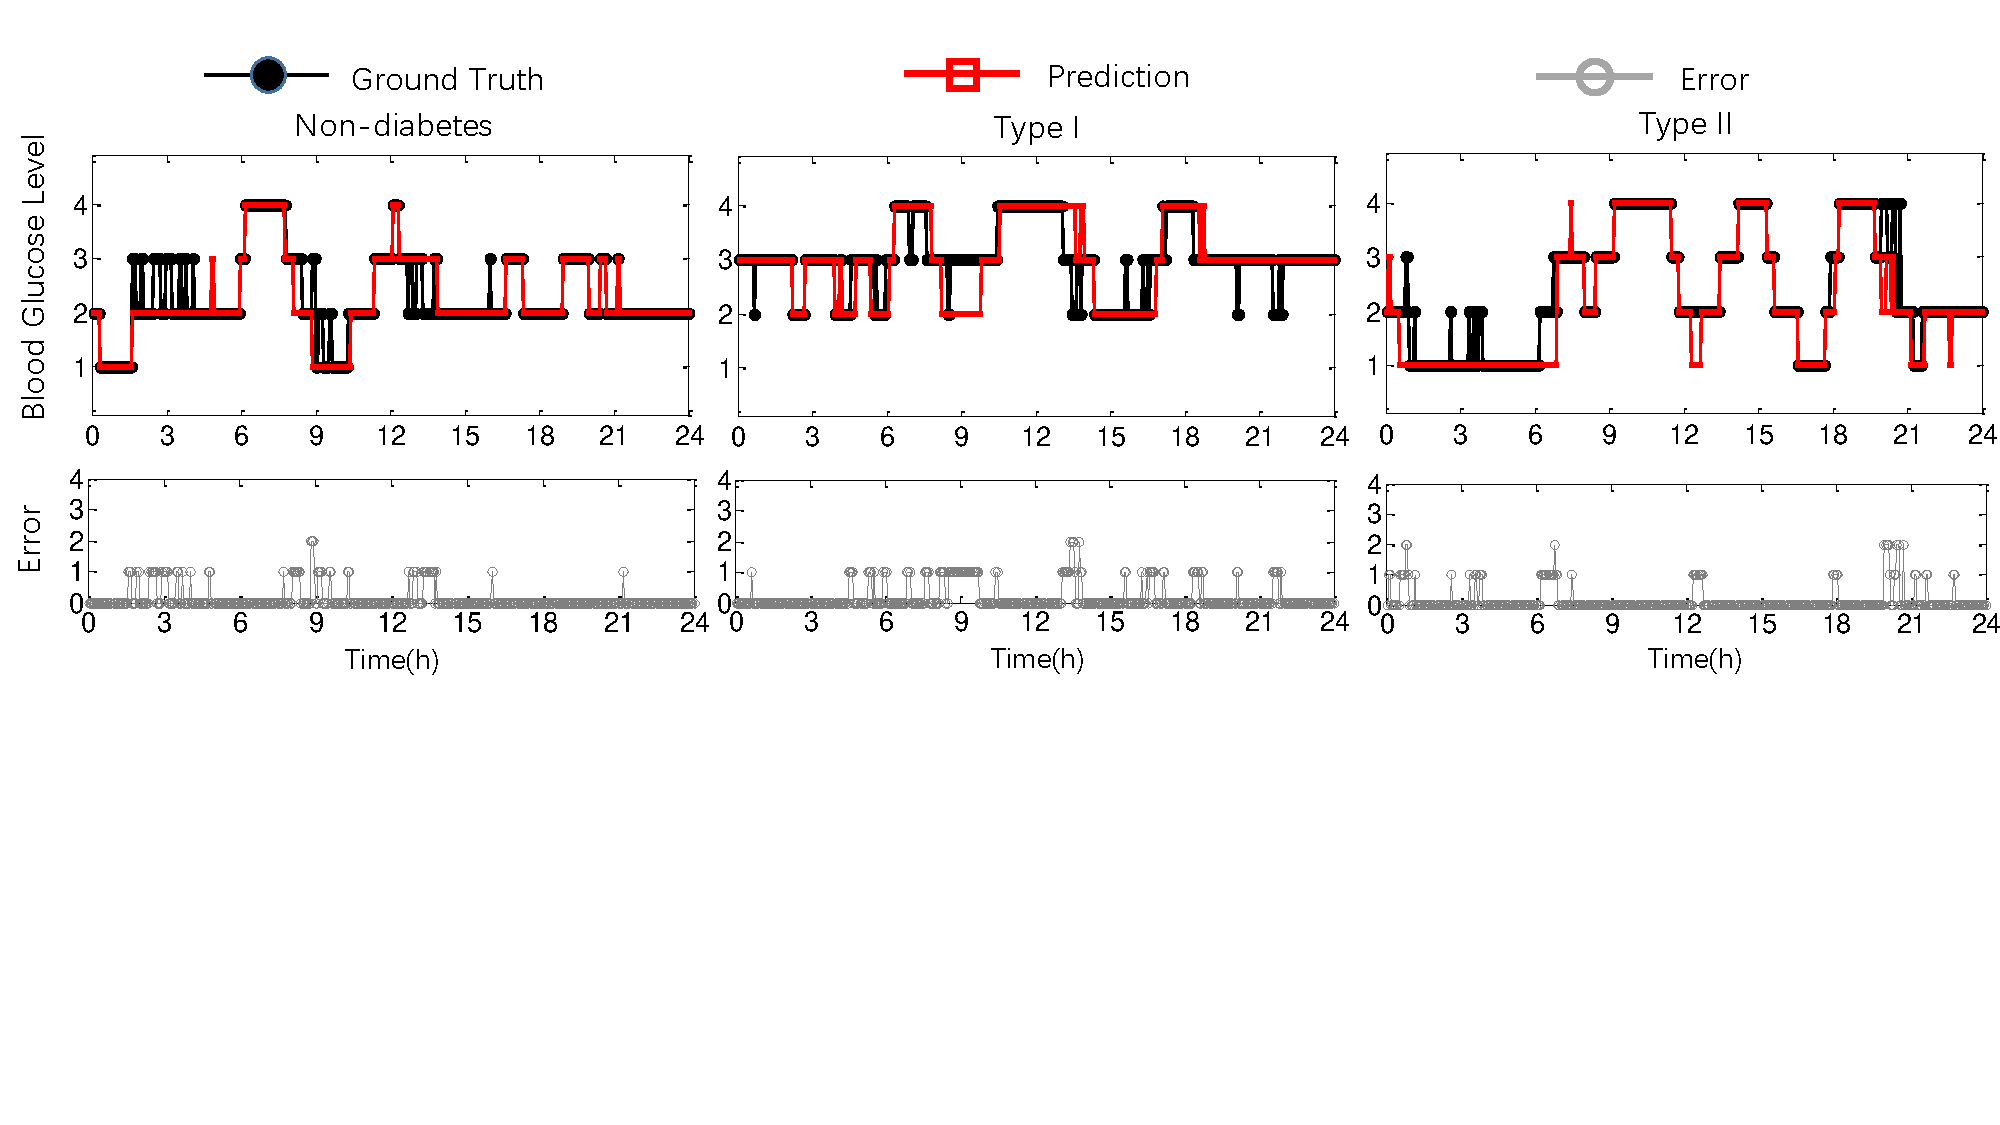
\includegraphics[width=0.5\columnwidth]{./img/pred_vs_gt.pdf}
\caption{The comparison of prediction and the ground truths of one user.}
\label{fig:pre_gt}
\end{figure}


\subsubsection{Model comparison}

We compare \modelname of \sysname over following baselines:

1) Gradient Boosting (GB): GB generates a prediction model by combining many weak classifiers into a stronger classification committee. We use AdaBoost procedure implemented in the fastAdaboost package to combine basic tree classifiers for ensemble learning. We vary the maximum tree depth from 10 to 50 by factors of ten. The number of boosting iterations is varied from 100 to 500 by a step size of 50.

2) Support Vehicle Machine (SVM): SVM bases on the idea of “optimal separating hyperplane” that maximizes the separation margin of two data groups (classes). Due to this construction, it usually generalizes well, and its dual form is a quadratic programing that can be easily incorporated with kernels. We train the Gaussian kernel SVM classifier with the kernlab package, which implements the sequential minimal optimization algorithm. We vary the kernel width from $2^{-5}$ to $2^4$ with a factor of 2. We pick the penalty parameter from the set $\{10^i | i = -3, 0.5, 2\}$. To eliminate scale/location discrepancies among input variables, all features are normalized before being used in the training phase.

3) Hidden Markov model (HMM):

4) Logistic Regression (LR): LR models the posterior distribution of the class labels as a sigmoidal function of linear combinations of features. We use the glmnet package to train LR models with elastic net (combined L1 and L2) regularization. We vary the penalty parameter from 10$^{-3}$ to 10$^2$ with a factor 5. The mixing parameter is varied from 0 (Ridge) to 1 (Lasso) by a step size of 0.1.

5) Random Forest (RF): As another ensemble method, RF combines many simple decision trees together and output the mode of classes for prediction. To avoid correlation among base trees, random set of features are selected in the splitting process when constructing each decision tree. For implementation, we adopt the conditional inference tree algorithm in the Party package. The total number of trees is tuned from 100 to 1000, and the maximum tree depth from 10 to 50. The splitting threshold is also varied from 0.1 to 0.9 with 0.1 intervals for cross validation.

6) Gaussian Processes (GP): Instead of directly parameterizing a latent function for classification, GP models it with a generic Gaussian process. The posterior of the process is updated with training data set, and is “squashed” through a logistic function for classification. We implement GP with the kernlab package, which includes several approximation algorithms for acceleration. We use the radial basis kernel and vary the kernel width from 2$^{-5}$ to 2$^4$ with an incremental factor of 2$^{0.5}$.






\rev{\section{Preliminary User study}
\label{sec:user_study}
In addition to validating the effectiveness of \modelname, this section presents the feedbacks of users on the design and user experience of \sysname.

\subsection{Procedure}
We distributed a semi-structured questionnaire to the 112 participants in \secref{sec:eval}.
All the participants were paid about 20 USD (in the local currency) after the survey.
We present the main results as follows\footnote{Not that most participants are not proficient in English. The original questionnaire was in the mouth tongue of the participants. The responses were carefully translated into English and presented in the results.}.

\subsection{Results}

\subsubsection{Operability of \sysname}
In this part of the survey, the participants were asked to rate the overall operability of \sysname as well as the three manual operations (food, drug and insulin intake) in three levels (\textit{Inconvenient}, \textit{Normal} and \textit{Convenient}).
The participants make comments on their practical operations. For example, those non-diabetic users who do not need to record drugs and insulin only rate the operation of food input, and the diabetic users who do not inject insulin are only report the comments on the food and drag inputs.
They were also required to express their opinions on the overall operability.

\begin{figure}[h]
  \centering
  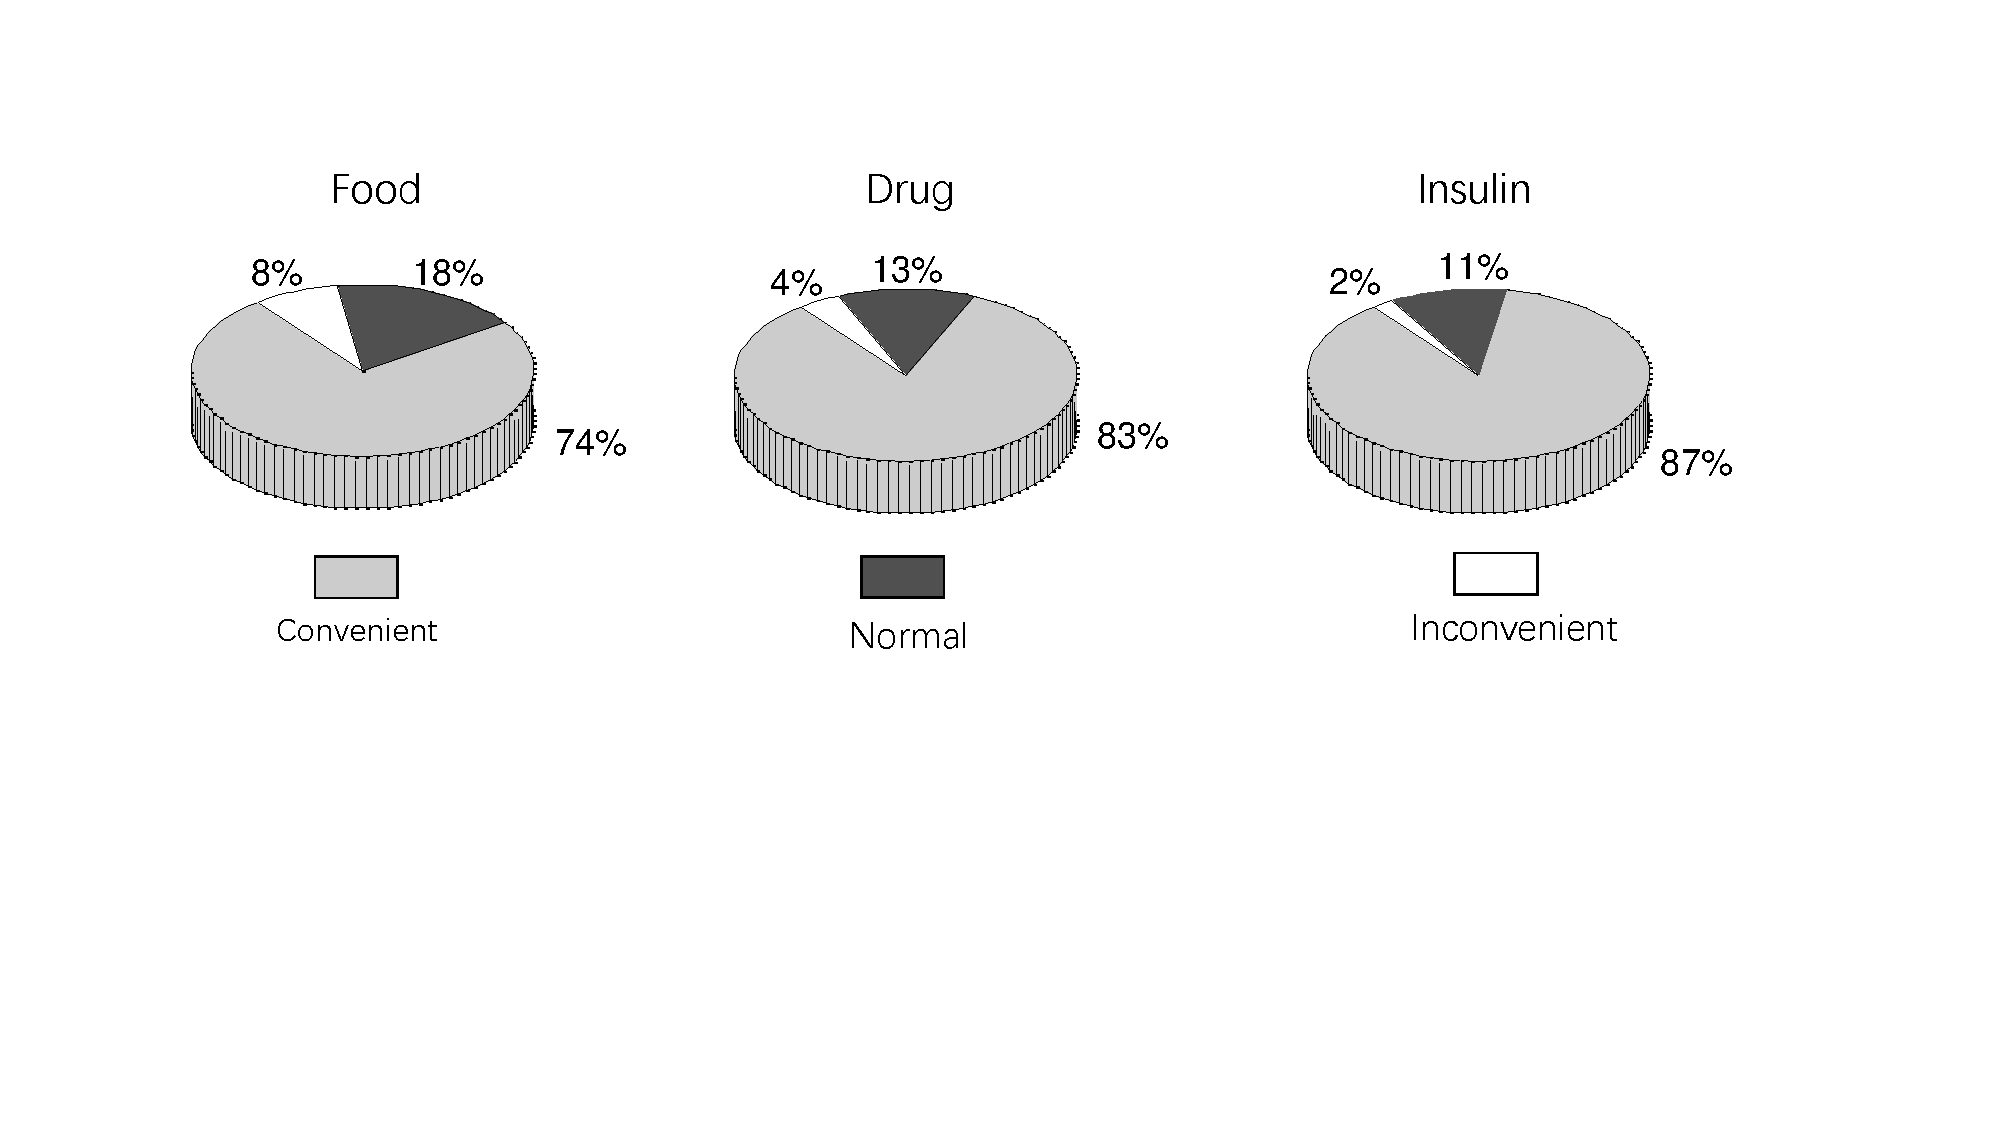
\includegraphics[width=0.8\columnwidth]{./img/user_cases.pdf}
  \caption{\rev{Distributions of user rating on the operability of food, drug and insulin intake recording interfaces.}}
  \label{fig:user_cases}
\end{figure}

\figref{fig:user_cases} illustrates the distributions of the user ratings on the operability of food, drug and insulin intake recording interfaces.
Overall, 78\%, 18\% and 4\% of the participants rate \sysname as \textit{Convenient}, \textit{Normal} and \textit{Inconvenient}, respectively.
The lowest rates are seen for manual recording of food intake (74\% as \textit{Convenient}).
The ratings for manual recording of drug and insulin intake are slightly better.
\TODO{present the results for the three groups of users separately, because non-diabetic users may not need to record drug and insulin intake, which leads them to give a higher rank.}

We select one representative comment for each level as follows:
\begin{itemize}
  \item
  \textit{``This App is easy to learn and quick to use.
  The database of food, drugs and insulin is very comprehensive.''}
  [Convenient, Type II diabetic user]
  \item
  \textit{``What I would like to see is a way to fill in the daily inputs by taking photos and speech.
  It would be more convenient to operate.''}
  [Normal, Type I diabetic user]
  \item
  \textit{``I don't have much time to record what I had for each meal using a scrolling menu.
  The App should be more personalized.
  For example, it should learn from my input history and provide search hints or automatic records.''}
  [Inconvenient, non-diabetic user]
\end{itemize}

As expected, the manual recording of food, drug and insulin intake tends to be a burden for \sysname as an intriguing application.
Nevertheless, we have collected some constructive suggestions from the users.
For instance, speech input instead of a scrolling menu might be a more welcome input mechanism.
Intelligent search hints based on personal input history using recommendation algorithms~\cite{bib:fu2000mining} may help to improve the user experience when recording food intake, which is highly diversified and challenging to record automatically.

\subsubsection{Benefits of \sysname}
In this part of the survey, each participant is asked to comment whether \sysname is useful by rating \sysname in three levels (\textit{Instructive}, \textit{Normal} and \textit{Non-instructive}) and commenting in detail.

94\% of the participants report \sysname as \textit{Instructive} and 6\% report \textit{Normal}.
No participant rates \sysname as \textit{Non-instructive}.
We also list two representative comments below.
\begin{itemize}
  \item
  \textit{``\sysname guides me to control my blood glucose and helps to live a healthier lifestyle.
  For instance, I always observe the blood glucose dynamics after meals.
  \sysname helps to figure out that my blood glucose rises a lot after I eat noodles, breads and dumplings, but stays relatively stable after eating meat and vegetables.
  Also I can learn about the impact of the drugs on my blood glucose.
  I'm happy to understand how my lifestyle affects my blood glucose and learn to make some adjustments in time.
  I have recommended \sysname to six friends.
  They also care about their blood glucose levels.''}
  [Instructive, Type II diabetic user]
  \item
  \textit{``I'm not diabetic but I feel I need to start tracking my blood glucose occasionally.
  This app has made it easy but still has room to improve.
  It presents me a short-term impact of food intake.
  However, I still care about how to maintain a long-term health status.
  Specifically, it should provide some suggestions to help me prevent developing into diabetes.''}
  [Normal, non-diabetic user]
\end{itemize}
In summary, users expect more functionalities of \sysname such as recommending intensity and time of exercises and recommending food plans.
In this regard, the personalized blood glucose dynamic records collected by \sysname can be sent to the experts to recommend personalized precaution measures.

\subsubsection{Willingness to use \sysname}
Finally, we are interested in whether the participants are willing to use \sysname for blood glucose tracking despite the manual input of food, drug and insulin intake.
In the questionnaire, we ask the following question:
\textit{``Are you willing to use \sysname instead of the CGM device if you need manual records of daily food, drug and insulin intake as well as wearing CGM for periodic re-calibration per month?''}
We also collect free-response comments as before.

\figref{fig:user_willingness} illustrates the results.
Over 90\% diabetic users (both Type I and Type II) are willing to use \sysname while non-diabetic users show a slightly lower willingness (85\%).
We also select two representative comments.
\begin{itemize}
  \item
  \textit{``
  Manual records seem much more convenience compared with wearing the CGM.
  I feel very uncomfortable when wearing the CGM.
  It reminds me that I am a patient all the time.
  Wearing the CGM device for calibration once a month is acceptable.
  At least 3/4 of the time I am free from the CGM device.''}
  [Willing, Type II diabetic user]
  \item
  \textit{``
  I am OK with the periodic CGM calibration, but the daily food record is a trouble for me.
  I always eat outside and easily forget what I have had after the meal.
  I'm not a patient.
  I don't like to record everything I did simply to track my blood glucose.''}
  [Unwilling, non-diabetic user]
\end{itemize}
From the feedbacks, it seems that most participants feel that continuous wearing of CGM devices is more uncomfortable.
Even if periodic re-calibration is required, many diabetic users think it is acceptable.
The manual recording of food intake is again the major concern, especially among non-diabetic participants.

\begin{figure}[h]
  \centering
  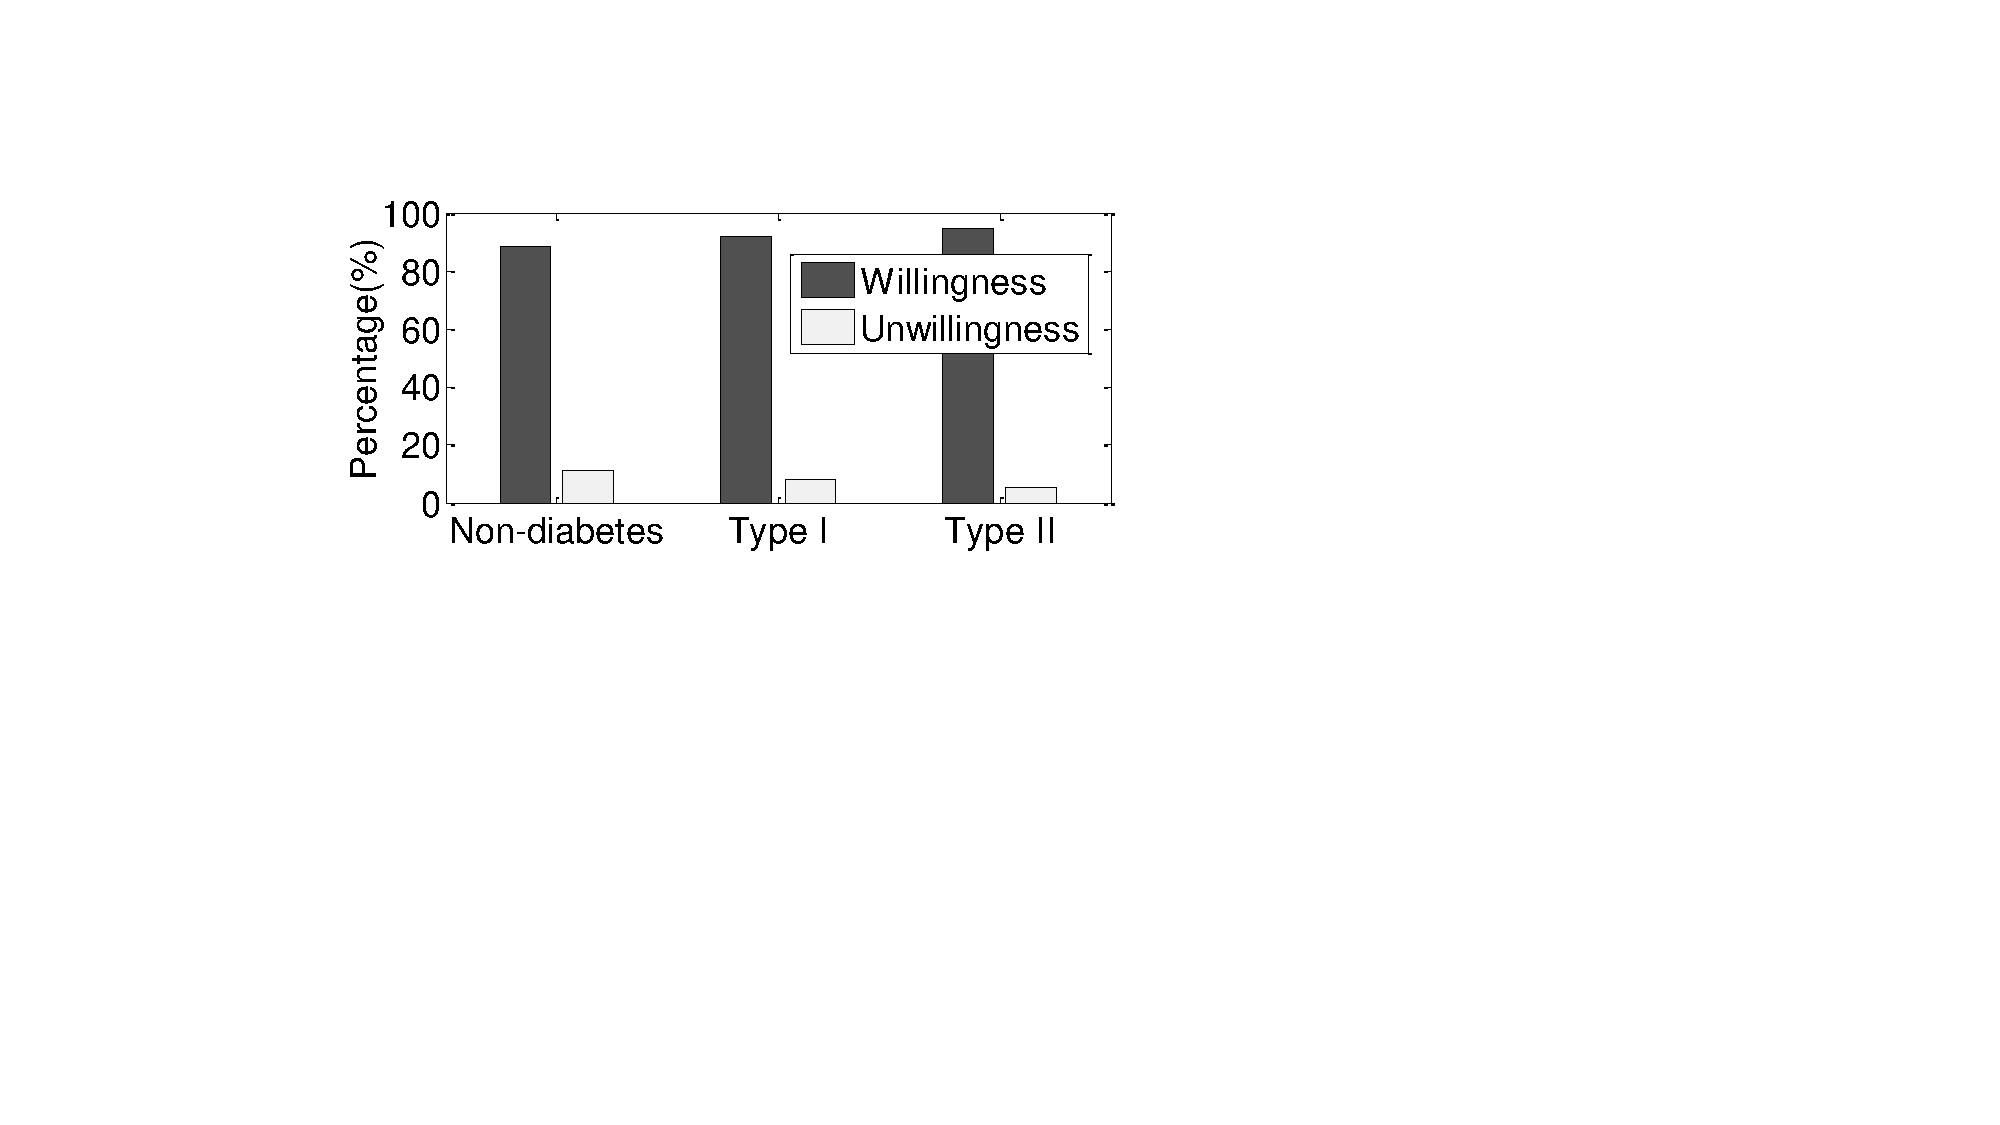
\includegraphics[width=0.4\columnwidth]{./img/willingness.pdf}
  \caption{\rev{Willingness to use \sysname.}}
  \label{fig:user_willingness}
\end{figure}


}

%\section{Discussion}
\label{sec:discussion}
\subsection{Usability}
\textcolor[rgb]{1.00,0.00,0.00}{This work focuses primarily on the challenges to monitor the blood glucose dynamics with few CGM calibration by the smartphones. A limitation of the existing prototype lies in collecting manually recorded data from users. As mentioned in section \ref{sec:user_study}, this issue can be handled with some current technologies such as computer vision \cite{bib:kawano2015foodcam}  and speech recognition \cite{bib:hinton2012deep}, and a camera API has been opened for users to take photos for their dishes, drug and insulin intake for the potential use. We are now optimizing the human-computing interaction on this side.}

\subsection{Inference error}
\textcolor[rgb]{1.00,0.00,0.00}{As mentioned in section~\ref{subsec:Inference_Results}, most errors come from two periods: 1) the transition of two blood glucose level 2) the duration of sudden blood glucose concentration change.
Based on the study of experiment, errors during blood glucose transitions are mainly brought by the temporary delays to measure the external factors. In this case, the inference result will follow up the true value in a short time once these external factors detected. Errors of sudden blood glucose fluctuation are often resulted by the abrupt or tiny changes of the external factors,
which may not be immediately detected by \sysname. In this case, the durations of errors are often too short to cause risky emergencies \cite{bib:Low_Blood_Glucose_(Hypoglycemia),bib:whitmer2009hypoglycemic}. In addition, 3.81\% Type D Clarke error in Table~\ref{predict_results} increases the false negative detection of blood glucose.
As mentioned in section~\ref{subsec:predict_result_analysis}, \sysname adopts a warning delay (9 mins) to copy with this issue. For the 0.91\% Type E error, it rarely happen and often occurs while the training and testing gap become large (more than 20 days). When the users find this case by double-check (finger sticker or CGM), we recommend users to wear CGM to collect data for periodic retraining. In the future, we will optimize the detection performance of \sysname to reduce these two types of errors.}


%Specifically, most errors belong to the results of Type B in \ref{subsec:predict_result_analysis}. }


\section{Conclusion}
\label{sec:conclusion}
Inferring blood glucose levels is important to avoid health risks incurred by hyperglycemia and hypoglycemia.
Commercial continuous blood glucose monitoring devices can be invasive and inconvenient to wear, which degrades the quality of life for diabetic patients and makes them inaccessible to non-diabetic people.
We present \sysname, a ubiquitous blood glucose level monitoring system using commodity smartphones.
It measures important external factors that affect blood glucose concentration and adopts machine learning to infer blood glucose levels at a fine-grained time resolution.
The core of \sysname is an efficient blood glucose learning paradigm, \modelname, which (1) depicts complex glucose dynamics via a deep RNN model, (2) extracts generic feature representations with a grouped multi-division framework, and (3) preserves individual differences using personalized outputs.
It tackles the sparsity and imbalance problem, which is the main hurdle of highly-accurate personalized blood glucose level tracking.
\rev{We deployed \sysname to 112 users and collect measurements at least 6 days from each person.}
Evaluations show that \modelname outperforms the state-of-the-arts methods on the blood glucose level inference.
With fully automatic recording of external factors in the future, we envision \sysname as a user-friendly and reliable complement for continuous blood glucose monitoring in daily life.

%Designing a pervasive and real-time blood glucose tracking system is crucial yet challenging. Existing devices either limited by the discontinuous usage (\eg finger pricking) or life interference (\ie continuous blood glucose monitor), preventing users measuring their blood glucose value regularly.
%The traditional inference models, however, suffer from the sparse data, resulting in the issue of low accuracy.
%In this paper, we implemented \sysname, a mobile framework tracking personal blood glucose level in real time.
%By adopting a novel statistical model \modelname, \sysname gets rid
%of the sparsity of individual blood glucose data, and then encodes the relationships between external factors and blood glucose levels comprehensively. The inference results could benefit users in learning their
%blood glucose alternation without interference, and further guiding their healthy behaviors (\eg the amount of food, drug and insulin intake, the sleep duration). We implemented \sysname on iOS platform and examined its performance on 112 participants over 7 months. The results show that \modelname outperforms the traditional statistical models, and achieves desirable monitor accuracy, making \sysname satisfy in daily use.


\bibliographystyle{ACM-Reference-Format}
\bibliography{sample-ubicomp}
\end{document}
%%% Local Variables:
%%% mode: latex
%%% TeX-master: t
%%% End:


